\documentclass[12pt]{article}
\usepackage[utf8]{inputenc}
\usepackage[english]{babel}
\usepackage[dotinlabels]{titletoc}
\usepackage{mathptmx}
\usepackage{amsmath, amssymb}
\usepackage{geometry, titlesec, setspace, enumitem}
\usepackage{xcolor, graphicx, caption, subcaption}
\usepackage{hyperref, natbib}
\usepackage{tabularx}
\usepackage{lipsum}
\usepackage{lmodern}
% Journals
\newcommand{\aap}{A\&A}
\newcommand{\aj}{AJ}
\newcommand{\apj}{ApJ}
\newcommand{\apjl}{ApJL}
\newcommand{\araa}{ARA\&A}
\newcommand{\mnras}{MNRAS}
\newcommand{\nat}{Nature}
\newcommand{\pasa}{PASA}
\newcommand{\pasp}{PASP}
\newcommand{\physrep}{PhR}
\newcommand{\prd}{PhRvD}
\newcommand{\rpph}{RPPh}

% Page formatting
\geometry{
	left=1.25in,
	right=1.25in,
	top=1in,
	bottom=1in}
\hypersetup{
	colorlinks=true,
	citecolor=blue,
	filecolor=blue,
	linkcolor=blue,
	urlcolor=blue
}
\setlength{\footnotesep}{10pt}
\setlist{noitemsep}

% Fixing titlesec and hyperref interaction
\makeatletter
\def\ttl@useclass#1#2{%
\@ifstar
{\ttl@labeltrue\@dblarg{#1{#2}}}
{\ttl@labeltrue\@dblarg{#1{#2}}}}
\makeatother

% Image setup
\graphicspath{{images/}}
\captionsetup[figure]{labelfont={bf}, font={small, stretch=1.3}, name={Figure}, labelsep=period}

% Section and subsection headings
\titleformat{\section}{\normalsize\bfseries\centering}{}{0em}{}
\titleformat{\subsection}{\normalsize\itshape\centering}{}{0.75em}{}
\newcommand{\nocontentsline}[3]{}
\newcommand{\tocless}[2]{\bgroup\let\addcontentsline=\nocontentsline#1{#2}\egroup}
\renewcommand{\contentsname}{Table of Contents}
\renewcommand{\abstractname}{{\normalsize\bfseries\centering{Abstract}}}
\renewcommand{\bibsection}{}

% For figures
\makeatletter
\setlength{\@fptop}{0pt plus 1fil}
\setlength{\@fpbot}{0pt plus 1fil}
\makeatother

% For formatting text and math
\let\vec\mathbf
\newcommand{\code}[1]{{\fontfamily{qcr}\selectfont#1}}
\newcommand{\red}[1]{\textcolor{red}{#1}}
\newcommand{\note}[1]{\textcolor{violet}{#1}}

% Special commands
\newcommand{\HI}{H\,\textsc{i}}
\newcommand{\OI}{O\,\textsc{i}}
\newcommand{\heraqm}{\code{hera\textunderscore qm}}
\newcommand{\herapspec}{\code{hera\textunderscore pspec}}
\newcommand{\herasim}{\code{hera\textunderscore sim}}
\newcommand{\pyuvdata}{\code{pyuvdata}}



\begin{document}
\doublespacing
\thispagestyle{empty}
\newpage
\pagenumbering{arabic}

\begin{center}
	{\Large \textbf{Estimating the Feasibility of Probing the Epoch of Reionization with the
									21cm-Ly$\alpha$ Cross-Power Spectrum}} \\
	[0.15\textheight]

	Prepared for: \\
	Drs. Daniel Jacobs (Director), Judd Bowman, \&  Philip Mauskopf\\
	Arizona State University \\
	School of Earth and Space Exploration \\[0.15\textheight]

	Prepared By: \\
	Tyler Cox \\
	Arizona State University \\
	School of Earth and Space Exploration \\
	Astrophysics Senior Thesis \\
	December 6$^{\textrm{th}}$ 2019 \\
	[0.15\textheight]

\end{center}
\thispagestyle{empty}

\clearpage
\pagenumbering{roman}

\begin{center}
	\textbf{Abstract}
\end{center}

asdf


\begingroup
\hypersetup{
	citecolor=DarkBlue,
	filecolor=black,
	linkcolor=black,
	urlcolor=DarkBlue
}
\renewcommand{\thesection}{\Roman{section}}
\tableofcontents
\listoffigures
\endgroup

\newpage

	\begin{center}
		\textbf{Acknowledgements}
	\end{center}

		First and foremost, I would like to thank the research advisors I've had since
I've joined the Low-Frequency Cosmology Lab (in no particular order), Adam Beardsley,
Judd Bowman, and Danny Jacobs. I am incredibly appreciative of your mentorship,
advice, and support.

Thank you to my third committee member, Alex Van Engelen, for enthusiastically
agreeing to sit on my committee despite the late notice.

I would also like to thank my friends, fellow students, and colleagues
who have made my time at ASU as enjoyable as it has been. In particular, I would like to
thank Shane Bechtel, Lily Whitler, and Samuel Nigh for their support and friendship.
I would also like to thank Lindsay Berkhout, Mrudula Gopalkrishna, Matt Kolopanis,
Steven Murray, and all of the members of the Low-Frequency Cosmology Lab.

Finally, I would like to send a heartfelt thank you to my parents and sister
for their constant love and encouragement.

\clearpage


\pagenumbering{arabic}


%----------------------------------%
%						Introduction					 %
%----------------------------------%

\tocless\section{\hypertarget{sec:introduction}{1\hspace{0.75em}Introduction}}
\addcontentsline{toc}{section}{1\hspace{0.75em}Introduction}

	\tocless\subsection{\hypertarget{subsec:universe}{1.1\hspace{0.75em}The Early Universe}}
	\addcontentsline{toc}{subsection}{1.1\hspace{0.75em}The Early Universe}

		Immediately following the Big Bang, the Universe was primarily composed of a hot plasma of fundamental particles. In its early state, it was  too hot and dense to form the atoms that form the complex structures that we observe today. Photons that were emitted during this early period scattered off free particles, leaving the Universe opaque to electromagnetic radiation. This lasted until roughly 400,000 years after the Big Bang, at which time the Universe had expanded and cooled sufficiently for electrons to bind to atomic nuclei forming the first atoms of hydrogen and helium. Once formed, photons were able to freely propagate through the intergalactic medium (IGM). Today, we observe this cosmic microwave background radiation (CMB).

\begin{figure}[th]
	\centering
	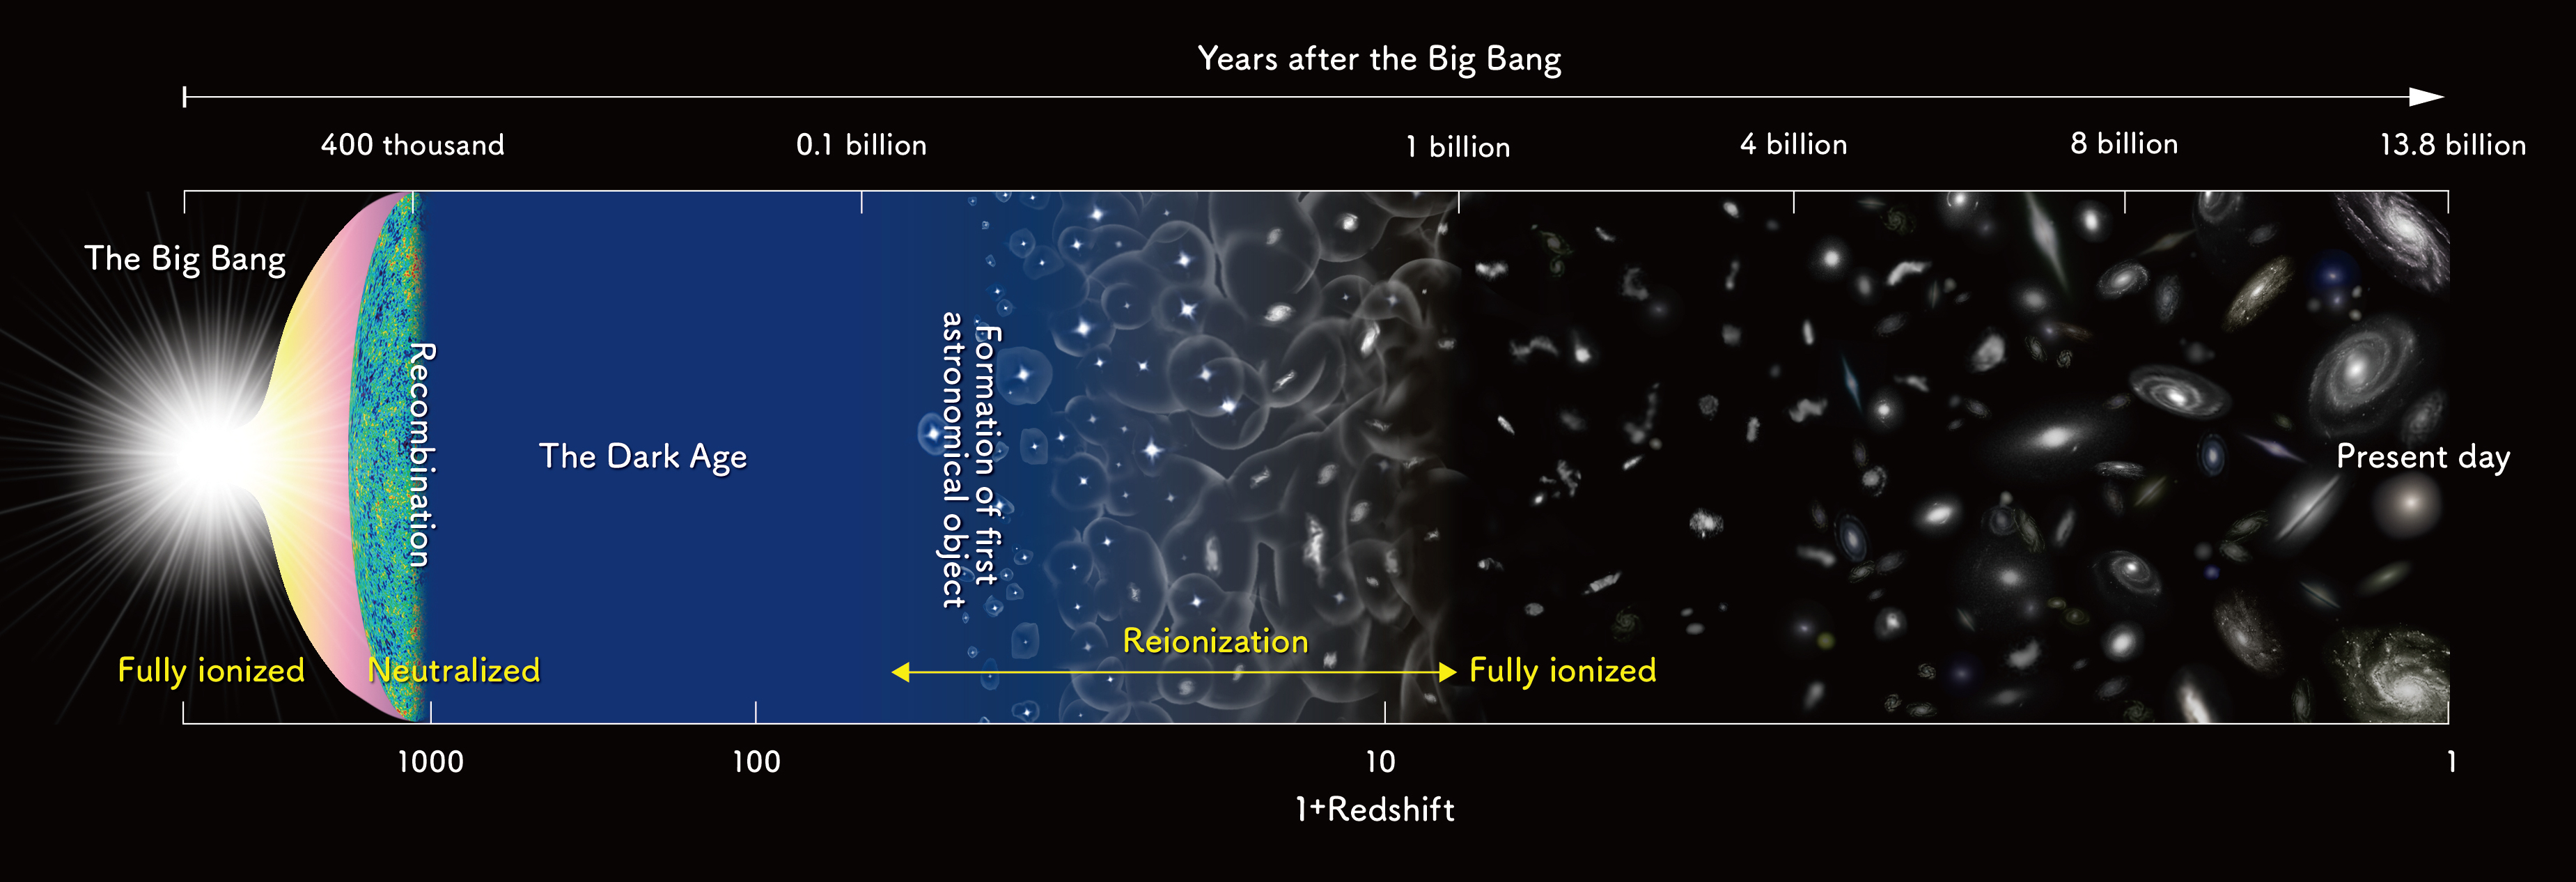
\includegraphics[width=1.0\textwidth]{intro/reionization.png}
	\caption[Epoch of Reionization Timeline]{Timeline of the history of the universe from its formation (left) to present day (right).}
	\label{fig:timeline}
\end{figure}

Following this recombination of matter, the universe was largely neutral and stationary.
Stars had not yet formed and the only emission detectable from this period originated
from neutral hydrogen. This period, called the Cosmic Dark Ages, lasted until roughly a few hundred millions after the Big Bang,
at which time the first luminous sources came into existence. Emitting ultraviolet (UV)
radiation, these first stars and galaxies began ionizing the neutral gas around them.
This period of time between the emergence of the first luminous sources and the
ionization of the neutral gas between them, named the Epoch of Reionization (EoR),
is believed to have lasted until around a billion years after the Big Bang.

Today, galaxies . Studying the EoR provides us the opportunity to establish a
bridge between the CMB and the structures we observe today, as well as provide
insight to what the first luminous objects were like and how they formed.


	\tocless\subsection{\hypertarget{subsec:eor}{1.2\hspace{0.75em}The Epoch of Reionization}}
	\addcontentsline{toc}{subsection}{1.2\hspace{0.75em}The Epoch of Reionization}

		

\begin{figure}[th]
	\centering
	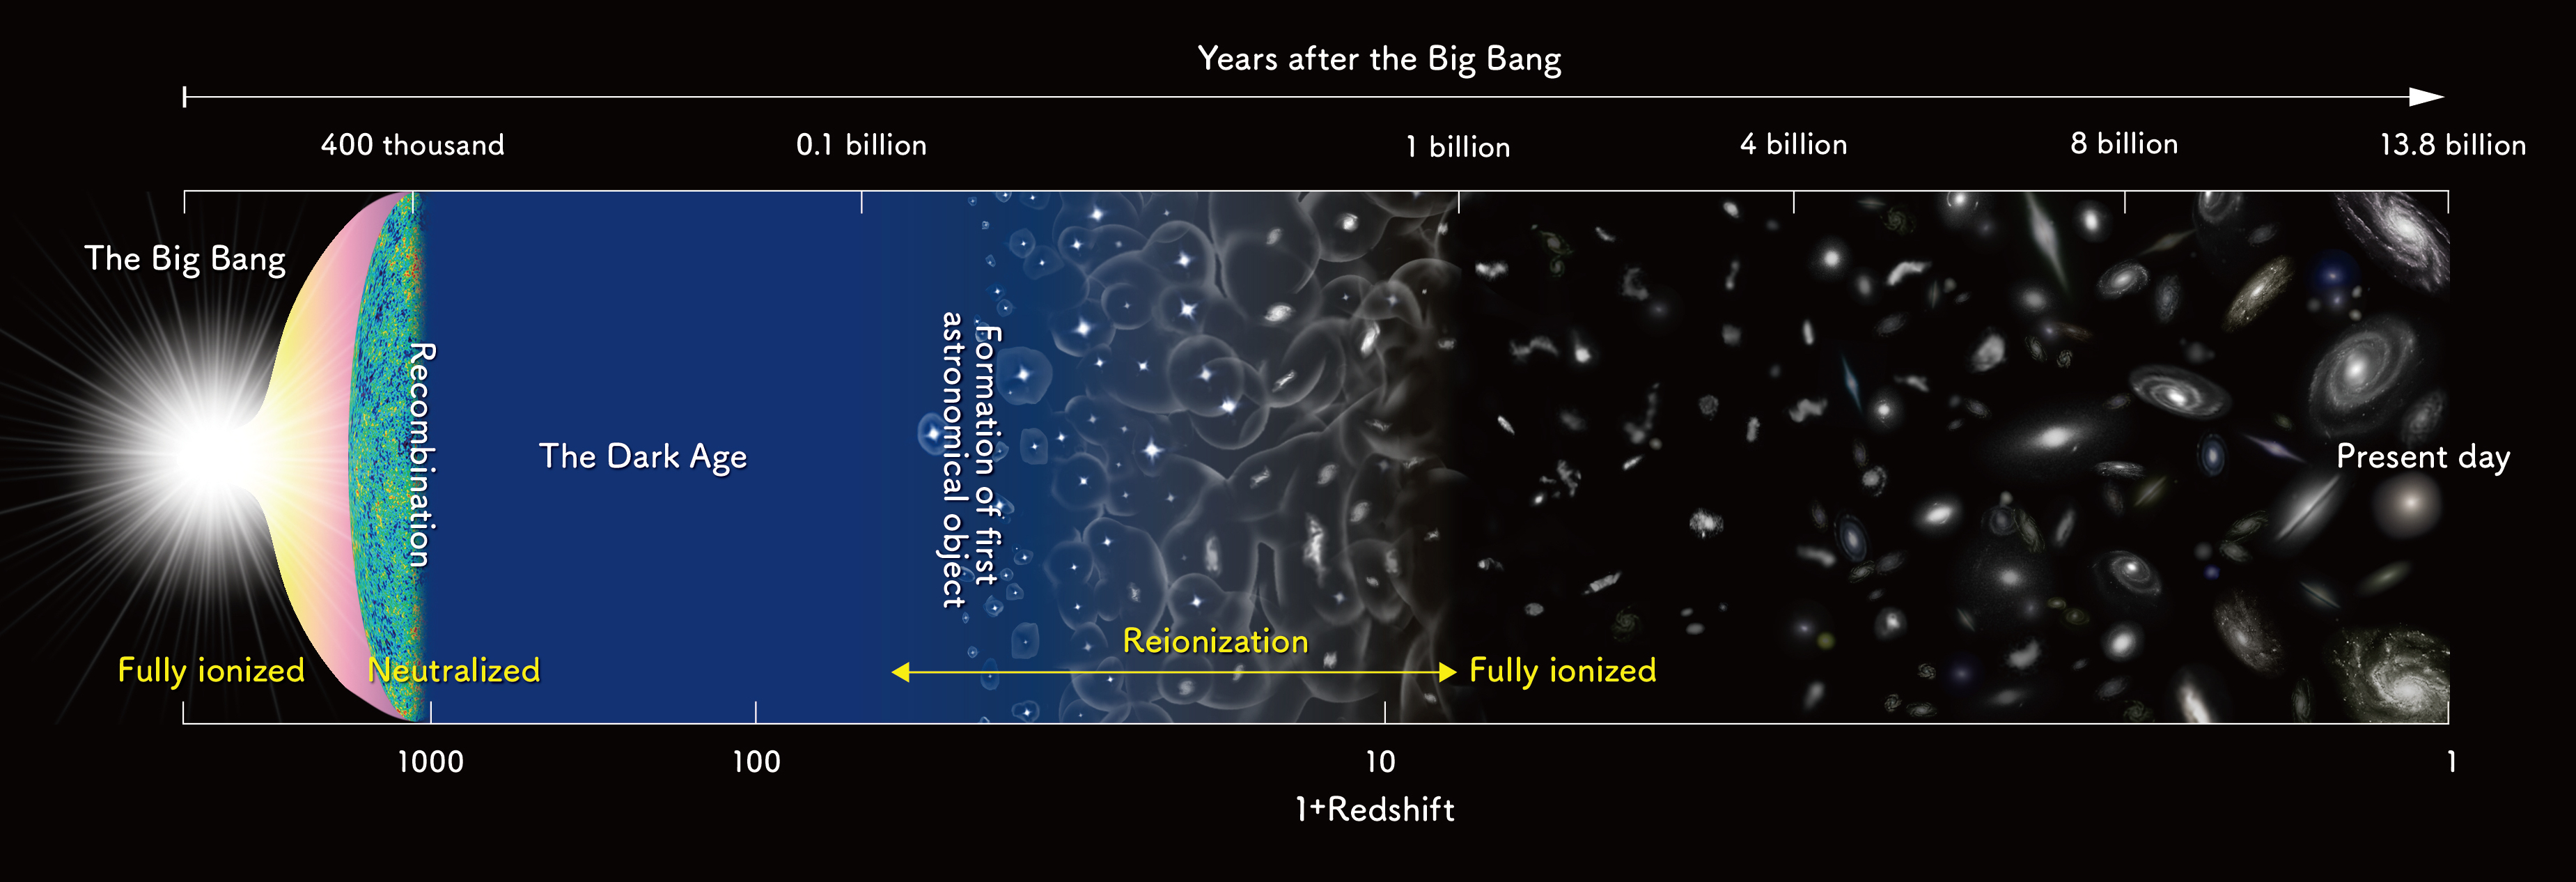
\includegraphics[width=1.0\textwidth]{intro/reionization.png}
	\caption[Epoch of Reionization Timeline]{Timeline of the history of the universe from its formation (left) to present day (right).}
	\label{fig:timeline}
\end{figure}



\begin{figure}[th]
	\centering
	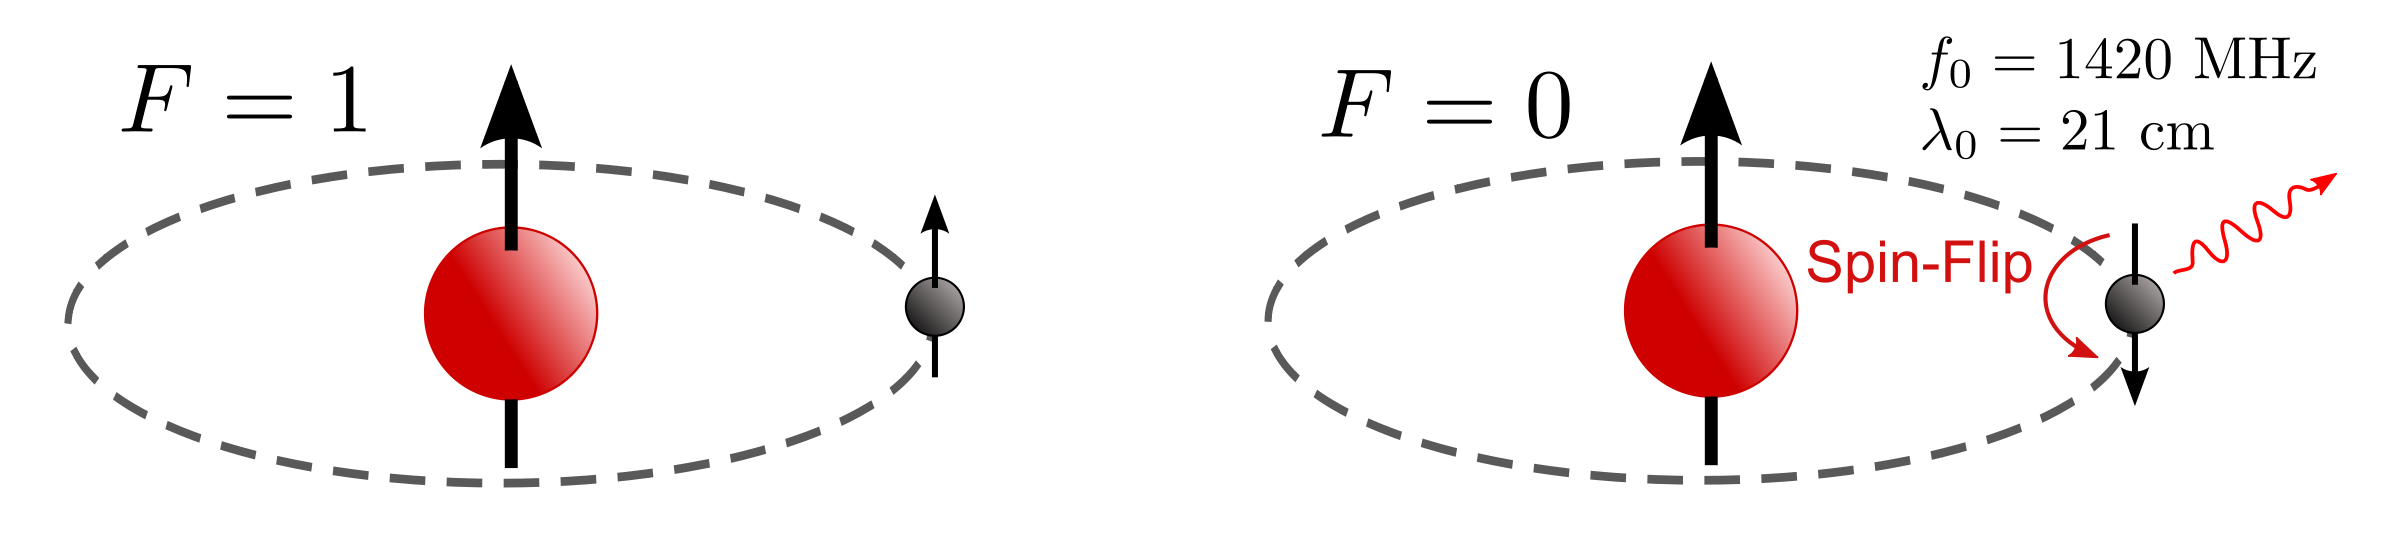
\includegraphics[width=0.90\textwidth]{spin_flip_H.png}
	\caption[Spin-Flip Transition of Neutral Hydrogen]{A depiction of the spin-flip transition of neutral hydrogen. Initially,
																					 the spin of the proton and electron are parallel and oriented
																					 in the same direction. The transition occurs when the electron's spin spontaneously
																					 flips from the higher energy parallel alignment to the lower energy anti-parallel alignment,
																					 releasing a photon with a wavelength of 21\,cm.}
	\label{fig:spin_flip}
\end{figure}

\begin{figure}[th]
	\centering
	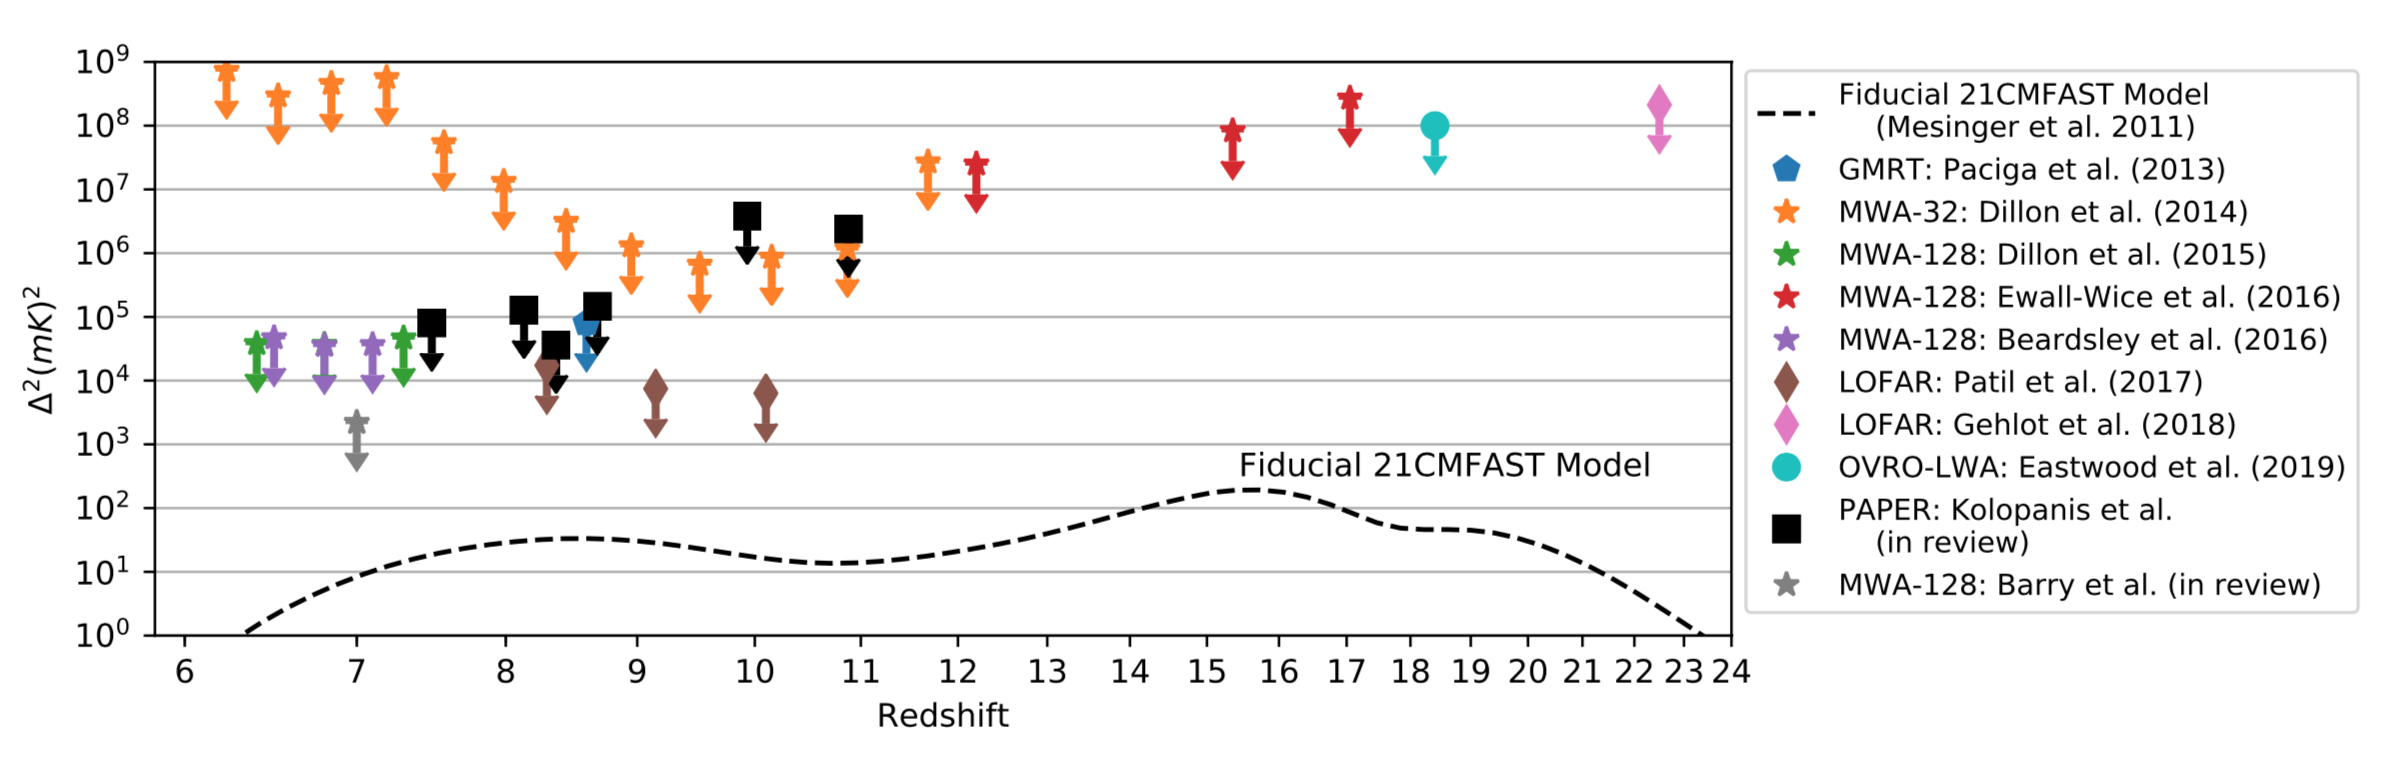
\includegraphics[width=1.\textwidth]{upper_limit.png}
	\caption[Upper Limits on Reionization]{A summary of the upper limits on the 21\,cm power spectrum across reionization. Plotted in the dashed line is a fiducial model of the 21\,cm power spectrum as simulated by \fastsim. Image taken from \cite{2019arXiv190708211L}}
	\label{fig:upper_limit}
\end{figure}


	\tocless\subsection{\hypertarget{subsec:hera}{1.3\hspace{0.75em}Intensity Mapping Experiments}}
	\addcontentsline{toc}{subsection}{1.3\hspace{0.75em}Intensity Mapping Experiments}

		\tocless\subsubsection{\hypertarget{subsubsec:hera}{1.3.1\hspace{0.75em}The Hydrogen Epoch of Reionization Array}}
		\addcontentsline{toc}{subsubsection}{1.3.1\hspace{0.75em}The Hydrogen Epoch of Reionization Array}

			\begin{figure}[th]
	\centering
	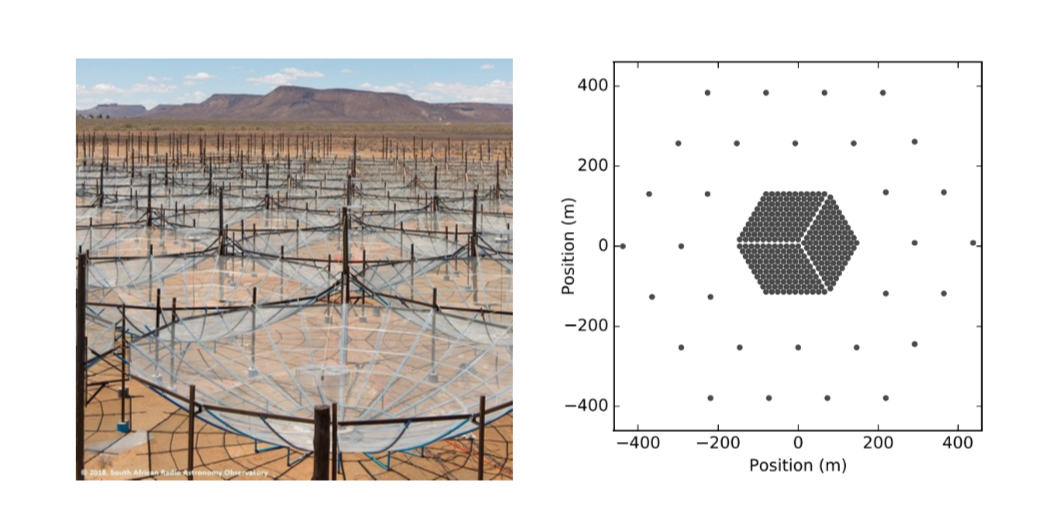
\includegraphics[width=0.95\textwidth]{intro/hera_layout.png}
	\caption[HERA Layout]{The power spectrum estimated after flagging a contiguous block of two channels.}
	\label{fig:hera_layout}
\end{figure}


\begin{figure}[th]
	\centering
	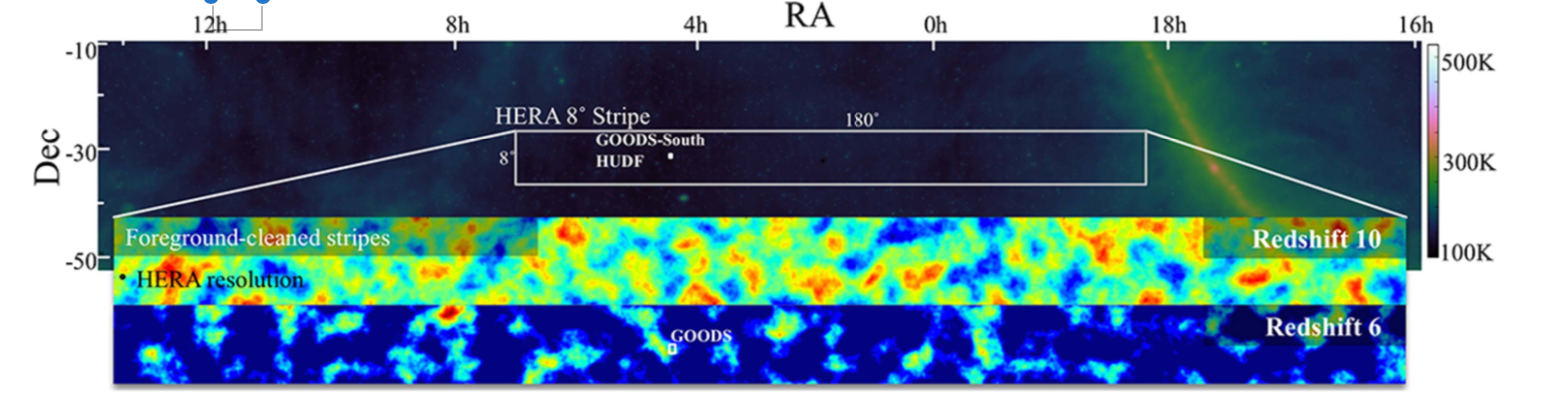
\includegraphics[width=0.95\textwidth]{intro/hera_stripe.png}
	\caption[HERA Field of View]{The power spectrum estimated after flagging a contiguous block of two channels.}
	\label{fig:hera_stripe}
\end{figure}


		\tocless\subsection{\hypertarget{subsec:spherex}{1.3.2\hspace{0.75em}SPHEREx}}
		\addcontentsline{toc}{subsubsection}{1.3.2\hspace{0.75em}SPHEREx}

			In addition using the 21\,cm line to characterize the EoR, intensity mapping of the
\lya\ transition of neutral hydrogen will provide a wealth of information about
the state of reionization. The \lya\ line has been shown to be a tracer of high-redshift
galaxies and the bubble of ionized gas around them in \cite{2013ApJ...763..132S} and \cite{2014ApJ...786..111P}.
A number of experiments look to probe reionization through the \lya\ line, but the most
prominent experiment of its kind planned for launch is that of the Spectro-Photometer
for the History of the Universe, Epoch of Reionization, and Ices Explorer (SPHEREx),
\cite{2014arXiv1412.4872D}.

\begin{figure}[th]
	\centering
	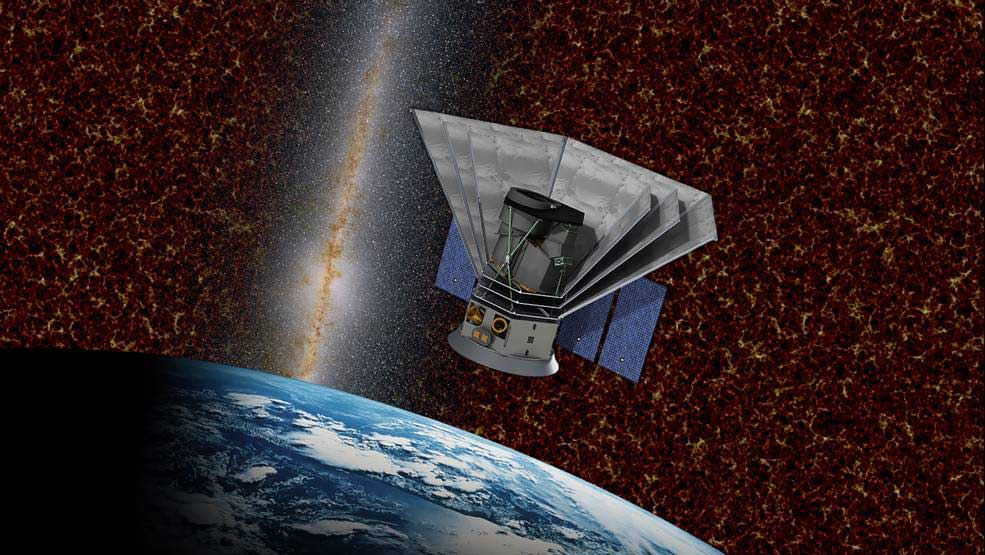
\includegraphics[width=0.95\textwidth]{spherex.jpg}
	\caption[SPHEREx Instrument]{Simulated image of the SPHEREx probe in orbit.}
	\label{fig:spherex}
\end{figure}

SPHEREx is a near-infrared, space-based observatory whose primary science goal is to perform
an all-sky survey in near-infrared bands of 450 million galaxies to constrain the
physics of inflation using the large-scale structure of these galaxies. While not
the primary goal of the mission, SPHEREx also looks to do intensity mapping of the
\lya\ line to study the origin and evolution of early galaxies. With a target launch
date set for December 2023, SPHEREx may provide the very first \lya\ intensity mapping
measurements during reionization. Given its sensitivity and frequency range, SPHEREx should
be able to detect these EoR fluctuations over the redshift range $z \approx 6 - 8$.


			\begin{figure}[th]
	\centering
	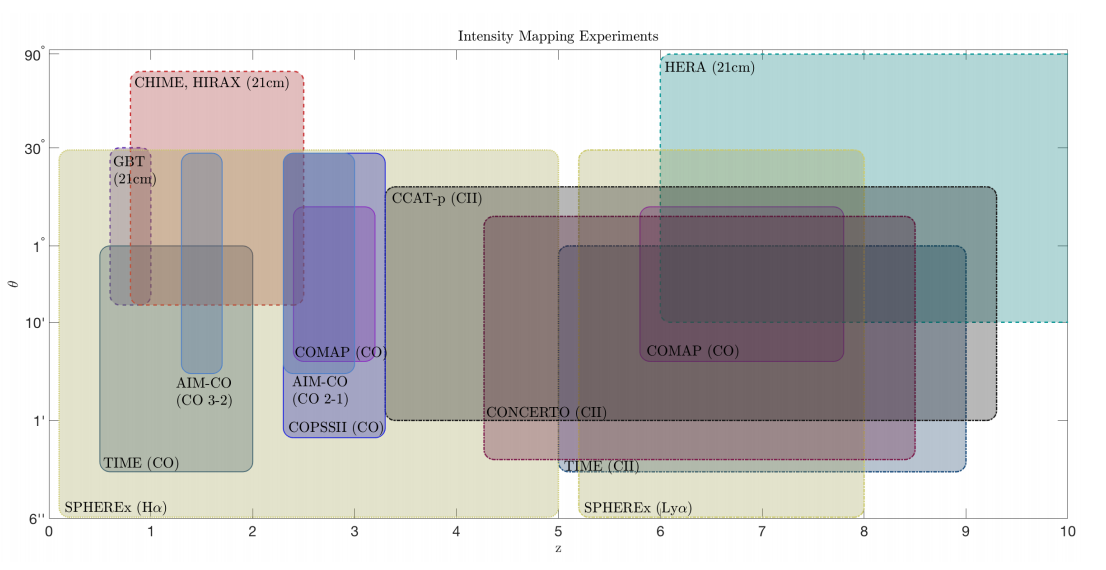
\includegraphics[width=0.95\textwidth]{results/intensity_mapping.png}
	\caption[Resolution and redshift of intensity mapping experiments]{}
	\label{fig:intensity_mapping}
\end{figure}





%----------------------------------%
%							Methods							 %
%----------------------------------%

\newpage

\tocless\section{\hypertarget{sec:methods}{2.\hspace{0.75em}Modeling 21cm and Ly$\alpha$ Fluctuations}}
\addcontentsline{toc}{section}{2.\hspace{0.75em}Modeling 21cm and Ly$\alpha$ Fluctuations}

	In this section, I will discuss the effort to model the 21\,cm and \lya\
cosmological signals that will be used for cross-correlation later in this work.
A significant amount of research has gone into the modeling effort of both 21\,cm and
\lya\ fluctuations during reionization. While N-body/radiative
transfer codes accurately capture the physics of the evolution of
galaxies and the IGM, they are computationally
expensive and are difficult to extend to the large cosmological volumes that HERA and SPHEREx will
attempt to observe. Semi-numerical simulators on the other hand are much more
computationally efficient at modeling the large-scale evolution of the IGM and
strongly agree with more numerically motivated simulators at the large scales that
these intensity mapping experiments are concerned with.
Additionally, computational efficiency is not only more convenient, but necessary
for later parameter studies.
For this work, I make use of the semi-numerical
simulator, \fastsim\ (\cite{2011MNRAS.411..955M}),
to simulate 21\,cm emission and to generate the density and ionization fields and halo catalogue
necessary for the simulation of \lya\ emission in later subsections.

Throughout this is work, I assume a flat, $\Lambda$CDM cosmology using cosmological
parameters consistent with \cite{2016A&A...594A..13P} and astrophysical
parameters defined in the \fastsim\ fidicual model. The physical comoving size of the
simulation cubes was $200 \times 200 \times 200 \ {\rm Mpc}^3$ with a voxel resolution
of 256 voxels on a side.


	\tocless\subsection{\hypertarget{subsec:methods}{2.1.\hspace{0.75em}21cm Fluctuations}}
	\addcontentsline{toc}{subsection}{2.1.\hspace{0.75em}21cm Fluctuations}

		\label{sec:21cm_temp}

In this subsection, I briefly describe the simulation of the 21\,cm cosmological
signal. As mentioned in the previously, \fastsim\ was written specifically to simulate the 21\,cm
signal. It does this by generating density, velocity, and ionization fields at $z \approx 35$ and evolving
them through cosmic time. With these fields and the following expression, the brightness temperature offset of the
21\,cm signal can then be evaluated at a given redshift.
\begin{align}
  \delta T_b \left(z \right) & = \frac{T_S - T_{\gamma}}{1+z} \left(1 - e^{-\tau_{\nu_0}} \right ) \nonumber \\
      & \approx 27 x_{\rm HI} \left( 1 + \delta_{\rm nl} \right) \left( \frac{H}{dv_r/dv + H}\right) \left( 1 - \frac{T_{\gamma}}{T_S}\right) \nonumber \\
      & \hspace{1em} \times \left( \frac{1 + z}{10} \frac{0.15}{\Omega_{\rm M} h^2} \right)^{1/2} \left( \frac{\Omega_{\rm b} h^2}{0.023} \right) \textrm{ mK,}
      \label{eqn:offset_temp}
\end{align}
In the equation above, $T_S$ is the gas spin temperature, $T_{\gamma}$ is the
CMB temperature, $\tau_{\nu_0}$ is the optical depth at 21cm frequency, $\delta_{\rm nl} = \rho / \bar{\rho}_0 - 1$
is the non-linear density contrast $H \left( z \right)$
is the Hubble parameter, $dv_r / dr$ is the comoving gradient of the line of sight component
of the comoving velocity, where all quantities are evaluated at redshift $z = \nu_0 / \nu - 1$.
The brightness temperature offset can then be converted to a fluctuation field
for cross-correlation using the equation below,
\begin{equation}
\delta_{21} \left( \mathbf{x}, z\right) = \frac{ \delta T_b \left( \mathbf{x}, z\right)}{\delta \overline{T}_b \left( z \right)} - 1,
\end{equation}
where $\delta \overline{T}$ is the spatial average of the 21\,cm brightness temperature offset
$\delta T \left( \mathbf{x}, z\right)$. The simulated 21\,cm brightness temperature offset field defined
in Equation \ref{eqn:offset_temp} can be see in Figure \ref{fig:sims}.


	\tocless\subsection{\hypertarget{subsec:methods}{2.2.\hspace{0.75em}Ly$\alpha$ Emission}}
	\addcontentsline{toc}{subsection}{2.2.\hspace{0.75em}Ly$\alpha$ Emission}

		Here I will describe the parameterization of \lya\ emission during reionization.
I adopt the techique developed in \cite{2013ApJ...763..132S} and applied in \cite{2017ApJ...848...52H}.
While modeling \lya\, I focus two locations from which \lya\ emission originates.

\begin{enumerate}
\item \textit{\lya\ Emitters (LAE)}: This is emission that originates from within the
              virial radius \lya\-emitting galaxies themselves. The dominate components
              that contribute to emission within these galaxies are hydrogen recombinations
              and collisional excitation.
\item \textit{Ionized Intergalactic Medium (IGM)}: This is emission that stems from the bubble
              of ionized gas that surround \lya\-emitting galaxies. In these ionized bubbles,
              X-ray/UV heating and scattering of Lyman-n photons as well as recombinations of
              ionized hydrogen are the dominate contributors to \lya\ emission.
\end{enumerate}


		\tocless\subsubsection{\hypertarget{subsubsec:methods}{2.2.1\hspace{0.75em}Galactic}}
		\addcontentsline{toc}{subsubsection}{2.2.1\hspace{0.75em}Galactic}

			\begin{equation}
\bar{I}_{\nu} = \int_{M_{\rm min}}^{M_{\rm max}} dM \frac{dn}{dM} I_{\nu} \left(M, z \right)
\end{equation}


		\tocless\subsubsection{\hypertarget{subsubsec:methods}{2.2.2\hspace{0.75em}Diffuse}}
		\addcontentsline{toc}{subsubsection}{2.2.2\hspace{0.75em}Diffuse}

			\label{sec:ionized_igm}

In this subsection, I describe the \lya\ emission from the ionized IGM. As mentioned
at the beginning of this section, I focus on \lya\ emission in the ionized IGM due to hydrogen recombinations.
As with \lya\ emitting galaxies, the ionized bubbles around galaxies also emits \lya\ photons through
recombinations of ionized hydrogen. The luminosity density of \lya\ emission in
some voxel of the simulation cubes can be defined using the following relationship,
\begin{equation}
  l_{\rm rec} = E_{\rm Ly\alpha} f_{\rm rec} \dot{n}_{\rm rec} \left( \textbf{x}, z \right),
\end{equation}
where $E_{\rm Ly\alpha}$ is the rest-frame energy of \lya\ photons, $f_{\rm rec}$ is the
fraction of recombinations that result in the emission of a \lya\ photon, and $\dot{n}_{\rm rec}$
is the comoving number density of recombinations occurring in the ionized IGM. The expression for the
number density of recombinations reads as,
\begin{equation}
  \dot{n}_{\rm rec} \left( \textbf{x}, z \right) = \alpha_{\rm A} n_{e} \left(z \right) n_{\textsc{HII}} \left(z \right),
\end{equation}
where $n_{e} = x_i \left( \textbf{x}, z \right) n_{b} \left( \textbf{x}, z \right)$,
$n_{\textsc{HII}} = n_{e} \left(4 - 4 Y_{\rm He} \right) /  \left(4 - 3 Y_{\rm He} \right)$ and $\alpha_{\rm A}$
is the comoving recombination coefficient. The comoving baryonic number density can be expressed using the
relationship below,
\begin{equation}
  n_{b} \left( \textbf{x}, z \right) = \bar{n}_{b, 0} \left( 1 + z\right)^3 \left[1 + \delta_{\rm nl} \left( \textbf{x}, z\right) \right],
\end{equation}
where $n_{b}$ is dependent on the non-linear density contrast, $\delta_{\rm nl} \left( \textbf{x}, z\right)$, and the
present-day mean baryonic number density, $\bar{n}_{b, 0} = 1.905 \times 10^{-7} \ \rm{cm}^{-3}$. Finally, the
comoving recombination coefficient, $\alpha_{\rm A}$, is defined below,
\begin{equation}
  \alpha_{\rm A} \approx 4.2 \times 10^{-13} \left( T_{\rm K} / 10^4 {\rm K} \right)^{-0.7} \left( 1 + z\right)^3 \ \left[\rm  cm^3 \ s^{-1} \right].
\end{equation}

The comoving number density of recombinations, $\dot{n}_{\rm rec}$, per pixel is simulated
by using \fastsim\ to evolve the kinetic gas temperature $T_k \left( \textbf{x}, z \right)$,
comoving baryonic number density $n_{b} \left( \textbf{x}, z \right)$, and the ionization
fraction $x_{i} \left( \textbf{x}, z \right)$ for each voxel in the simulation cube.
With the number density of recombinations calculated in each voxel, the luminosity
density of \lya\ emission in the ionized IGM can be calculated and converted to
a surface brightness using the following relationship,
\begin{equation}
I_{\nu}^{\rm rec} = y \left(z \right) d_A^2 \left(z \right) \frac{l_{\rm rec} \left( \textbf{x}, z \right)}{4 \pi d_L^2 \left( z \right)}.
\end{equation}

In reality, \lya\ emission from the ionized IGM also includes the scattered IGM \lya\
background whose main contributors are X-ray and UV heating, as well as the scattering of Lyman-n
photons emitted from galaxies by residual neutral hydrogen in the ionized IGM (\cite{2007MNRAS.376.1680P}).
For this work, I chose to neglect the contribution from this \lya\ background as its contribution
is subdominant to hydrogen recombination in the ionized IGM (roughly half the mean surface brightness)
and the galactic \lya\ contribution (about an order of magnitude lower) as found in \cite{2013ApJ...763..132S} and
\cite{2017ApJ...848...52H}. Adding in
the \lya\ background contribution in the future should be
trivial as \fastsim\ keeps track of this its emission when evolving the kinetic
gas temperature and the ionization field. The surface brightness
of \lya\ emission due to this background, $J_{\alpha} \left( \textbf{x}, z\right)$, can then be
calculated using the following expression (\cite{2013ApJ...763..132S}):

\begin{equation}
  I_{\nu} = \frac{6 E_{\text{Ly}\alpha}\, d_\textsc{a}^2 \left(z \right)}{\left( 1 + z\right)^2 d_\textsc{l}^2 \left( z \right)}\, J_{\alpha} \left( \textbf{x}, z \right).
\end{equation}

With all of the components of \lya\ emission during the EoR simulated and converted to surface brightnesses,
I then calculate the fluctuation field of \lya\ emission by summing over the individual
contributions to \lya\ emission from galaxies and the ionized IGM.
\begin{equation}
  \delta I_{\nu} \left(\textbf{x}, z \right) = \sum_i \frac{\nu I_{\nu, i} \left(\textbf{x}, z \right)}{\nu \bar{I}_{\nu} \left(z \right)} - 1
\end{equation}
This expression will to used to calculate the \lya\ auto-power spectrum and the 21\,cm-\lya\
cross-power spectrum in the following section. The slices through the simulated 21\,cm and the various
components of \lya\ emission cubes are shown in Figure \ref{fig:sims}.

\begin{figure}[p]
	\centering
	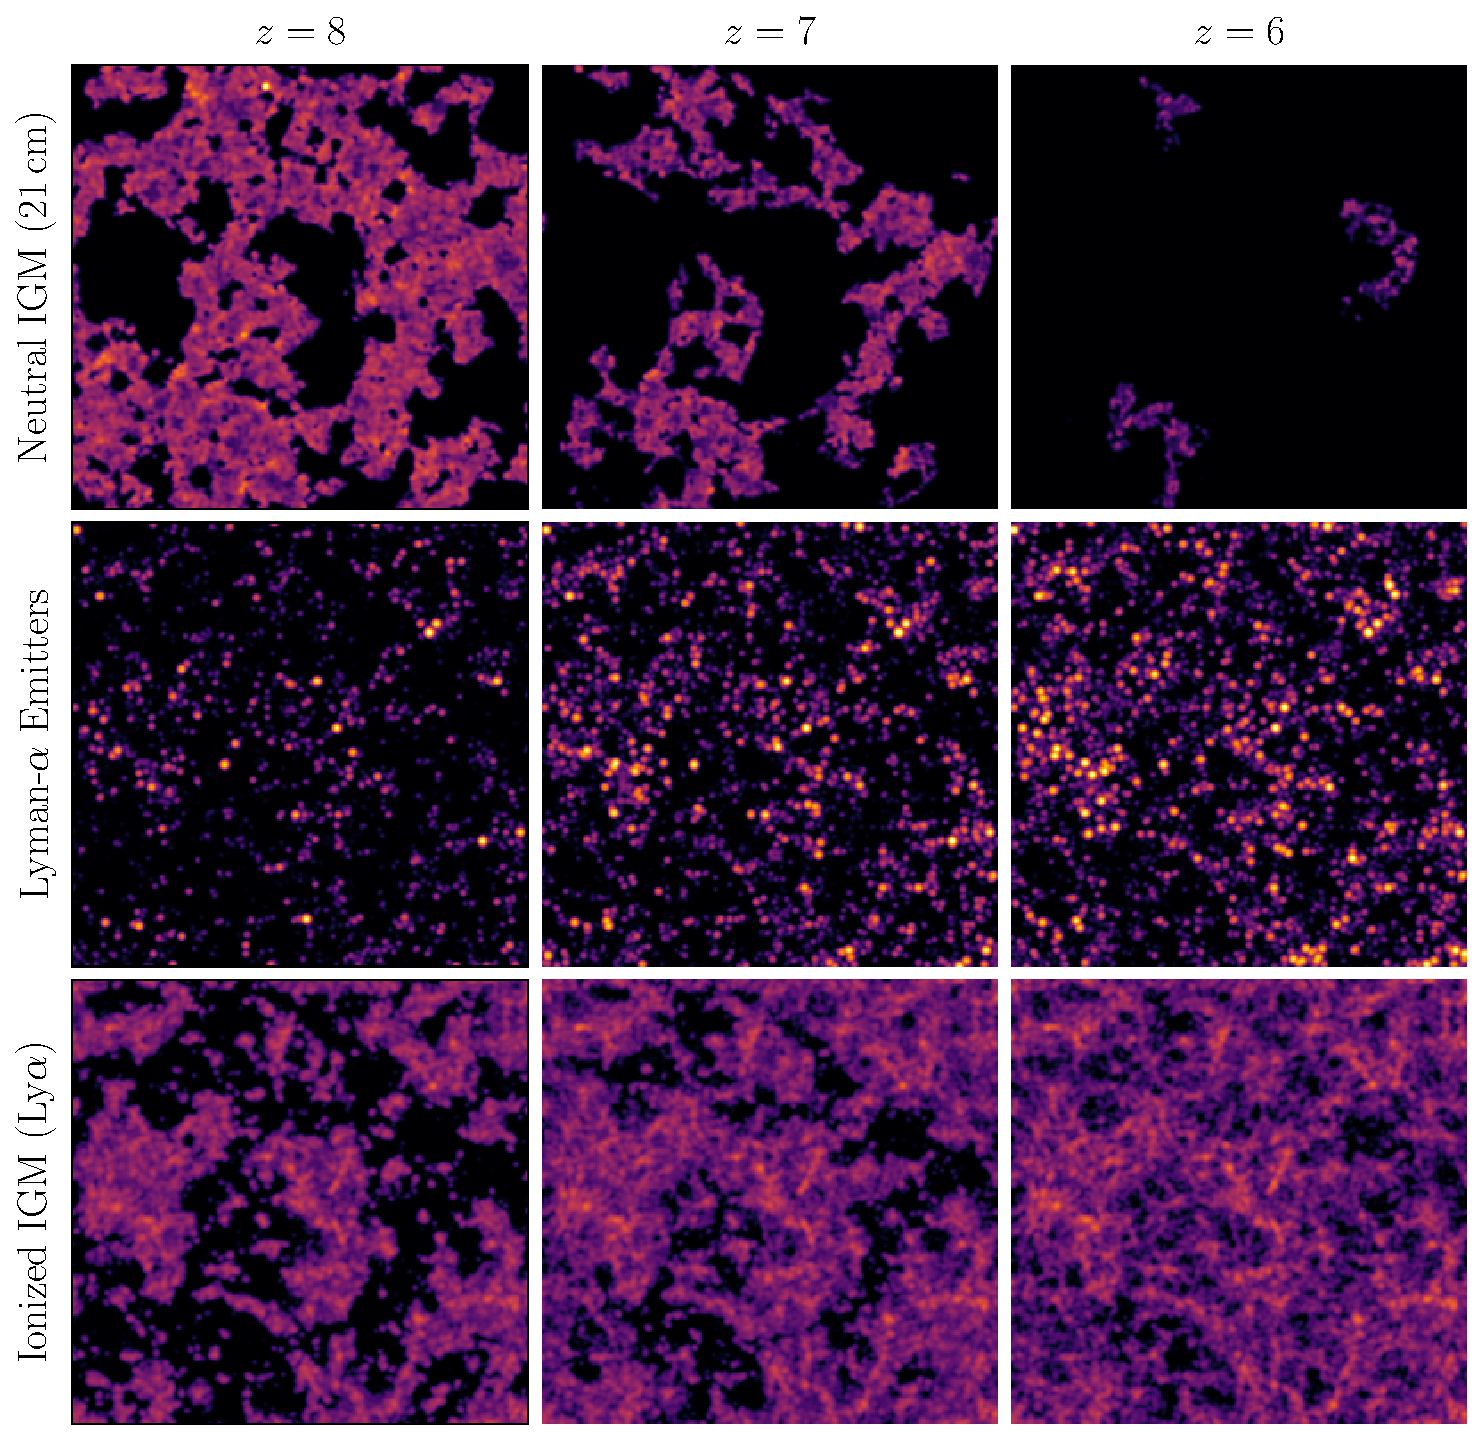
\includegraphics[width=1\textwidth]{sims.pdf}
	\caption[Simulated 21cm and \lya\ emission]{Slices through the simulated 21\,cm brightness temperature offset, $\delta T_b$, \lya\ emitter and ionized IGM cubes at $z = \left[6, 7, 8\right]$. Details on these simulations are described in Sections \hyperref[sec:21cm_temp]{2.1}, \hyperref[ref:laes]{2.2.1}, \hyperref[sec:ionized_igm]{2.2.2} respectively. The simulated box length is 200\,Mpc on a side. These fluctuation fields are used in later sections (Section \hyperref[sec:cross-power]{3.1}) to calculate the 21\,cm-\lya\ cross-power spectrum.}
	\label{fig:sims}
\end{figure}


		\tocless\subsubsection{\hypertarget{subsubsec:methods}{2.2.3\hspace{0.75em}Scattered}}
		\addcontentsline{toc}{subsubsection}{2.2.3\hspace{0.75em}Scattered}

			\begin{equation}
  I_{\nu} = \frac{6 E_{\text{Ly}\alpha}\, d_\textsc{a}^2 \left(z \right)}{\left( 1 + z\right)^2 d_\textsc{l}^2 \left( z \right)}\, J_{\alpha} \left( \textbf{x}, z \right)
\end{equation}


\begin{equation}
  \delta I_{\nu} \left(\textbf{x}, z \right) = \sum_i \frac{\nu I_{\nu, i} \left(\textbf{x}, z \right)}{\nu \bar{I}_{\nu, i} \left(z \right)} - 1
\end{equation}




\newpage

%----------------------------------%
%							Results							 %
%----------------------------------%

\tocless\section{\hypertarget{sec:results}{3.\hspace{0.75em}Cross-Correlation Studies}}
\addcontentsline{toc}{section}{3.\hspace{0.75em}Cross-Correlation Studies}

	\tocless\subsection{\hypertarget{subsec:results}{3.1.\hspace{0.75em}Cross-Power Spectrum}}
	\addcontentsline{toc}{subsection}{3.1.\hspace{0.75em}Cross-Power Spectrum}

		\begin{equation}
\langle \widetilde{\delta}_i ({\bf k}) \widetilde{\delta}_j ({\bf k'}) \rangle = (2 \pi) ^3 \delta_D \left( {\bf k} - {\bf k'} \right) P_{ij} \left({\bf k} \right)
\end{equation}

\begin{equation}
    \widetilde{\Delta} \left( k \right) = \frac{k^3}{2 \pi ^2} P \left( k \right)
\end{equation}

\begin{equation}
    \Delta \left( k \right) = \left( \nu I_{\nu} \right)^2 \widetilde{\Delta} \left( k \right)
\end{equation}s

\begin{figure}[ht]
	\centering
	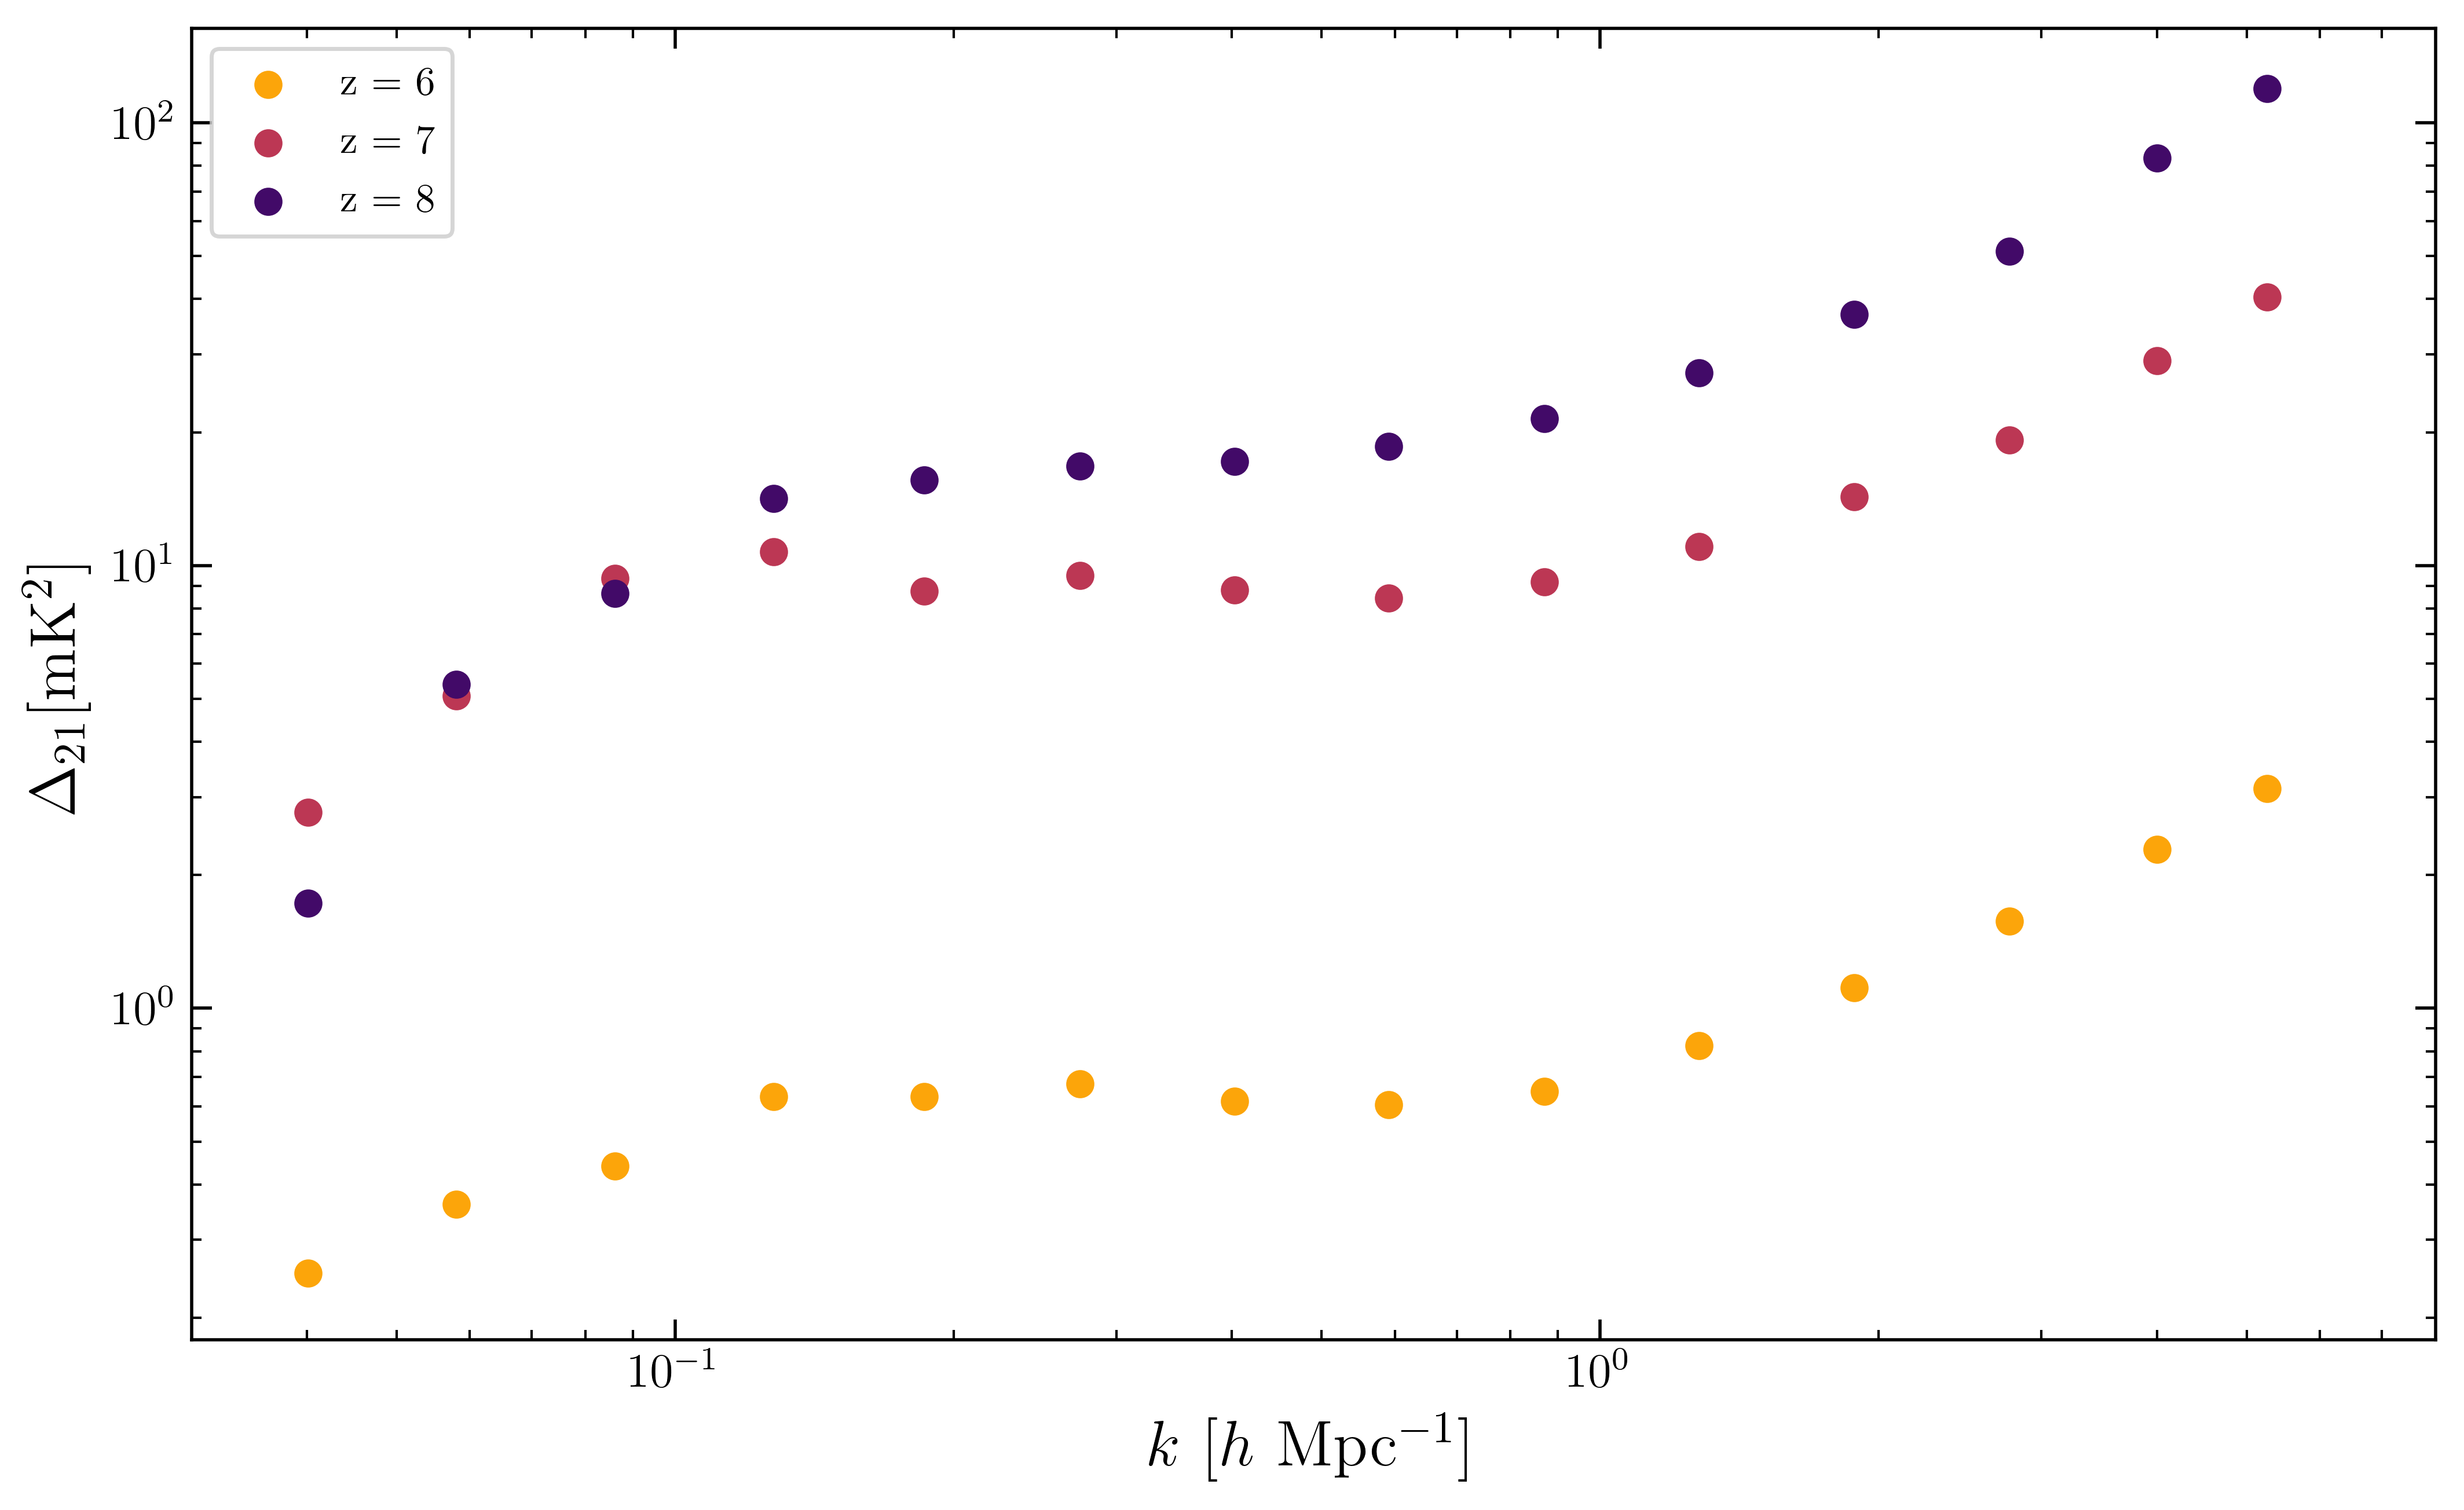
\includegraphics[width=0.9\textwidth]{21cm_power_spectrum.png}
	\caption[21cm Power Spectrum]{Cross-correlation coefficient}
	\label{fig:21cm_ps}
\end{figure}

\begin{figure}[ht]
	\centering
	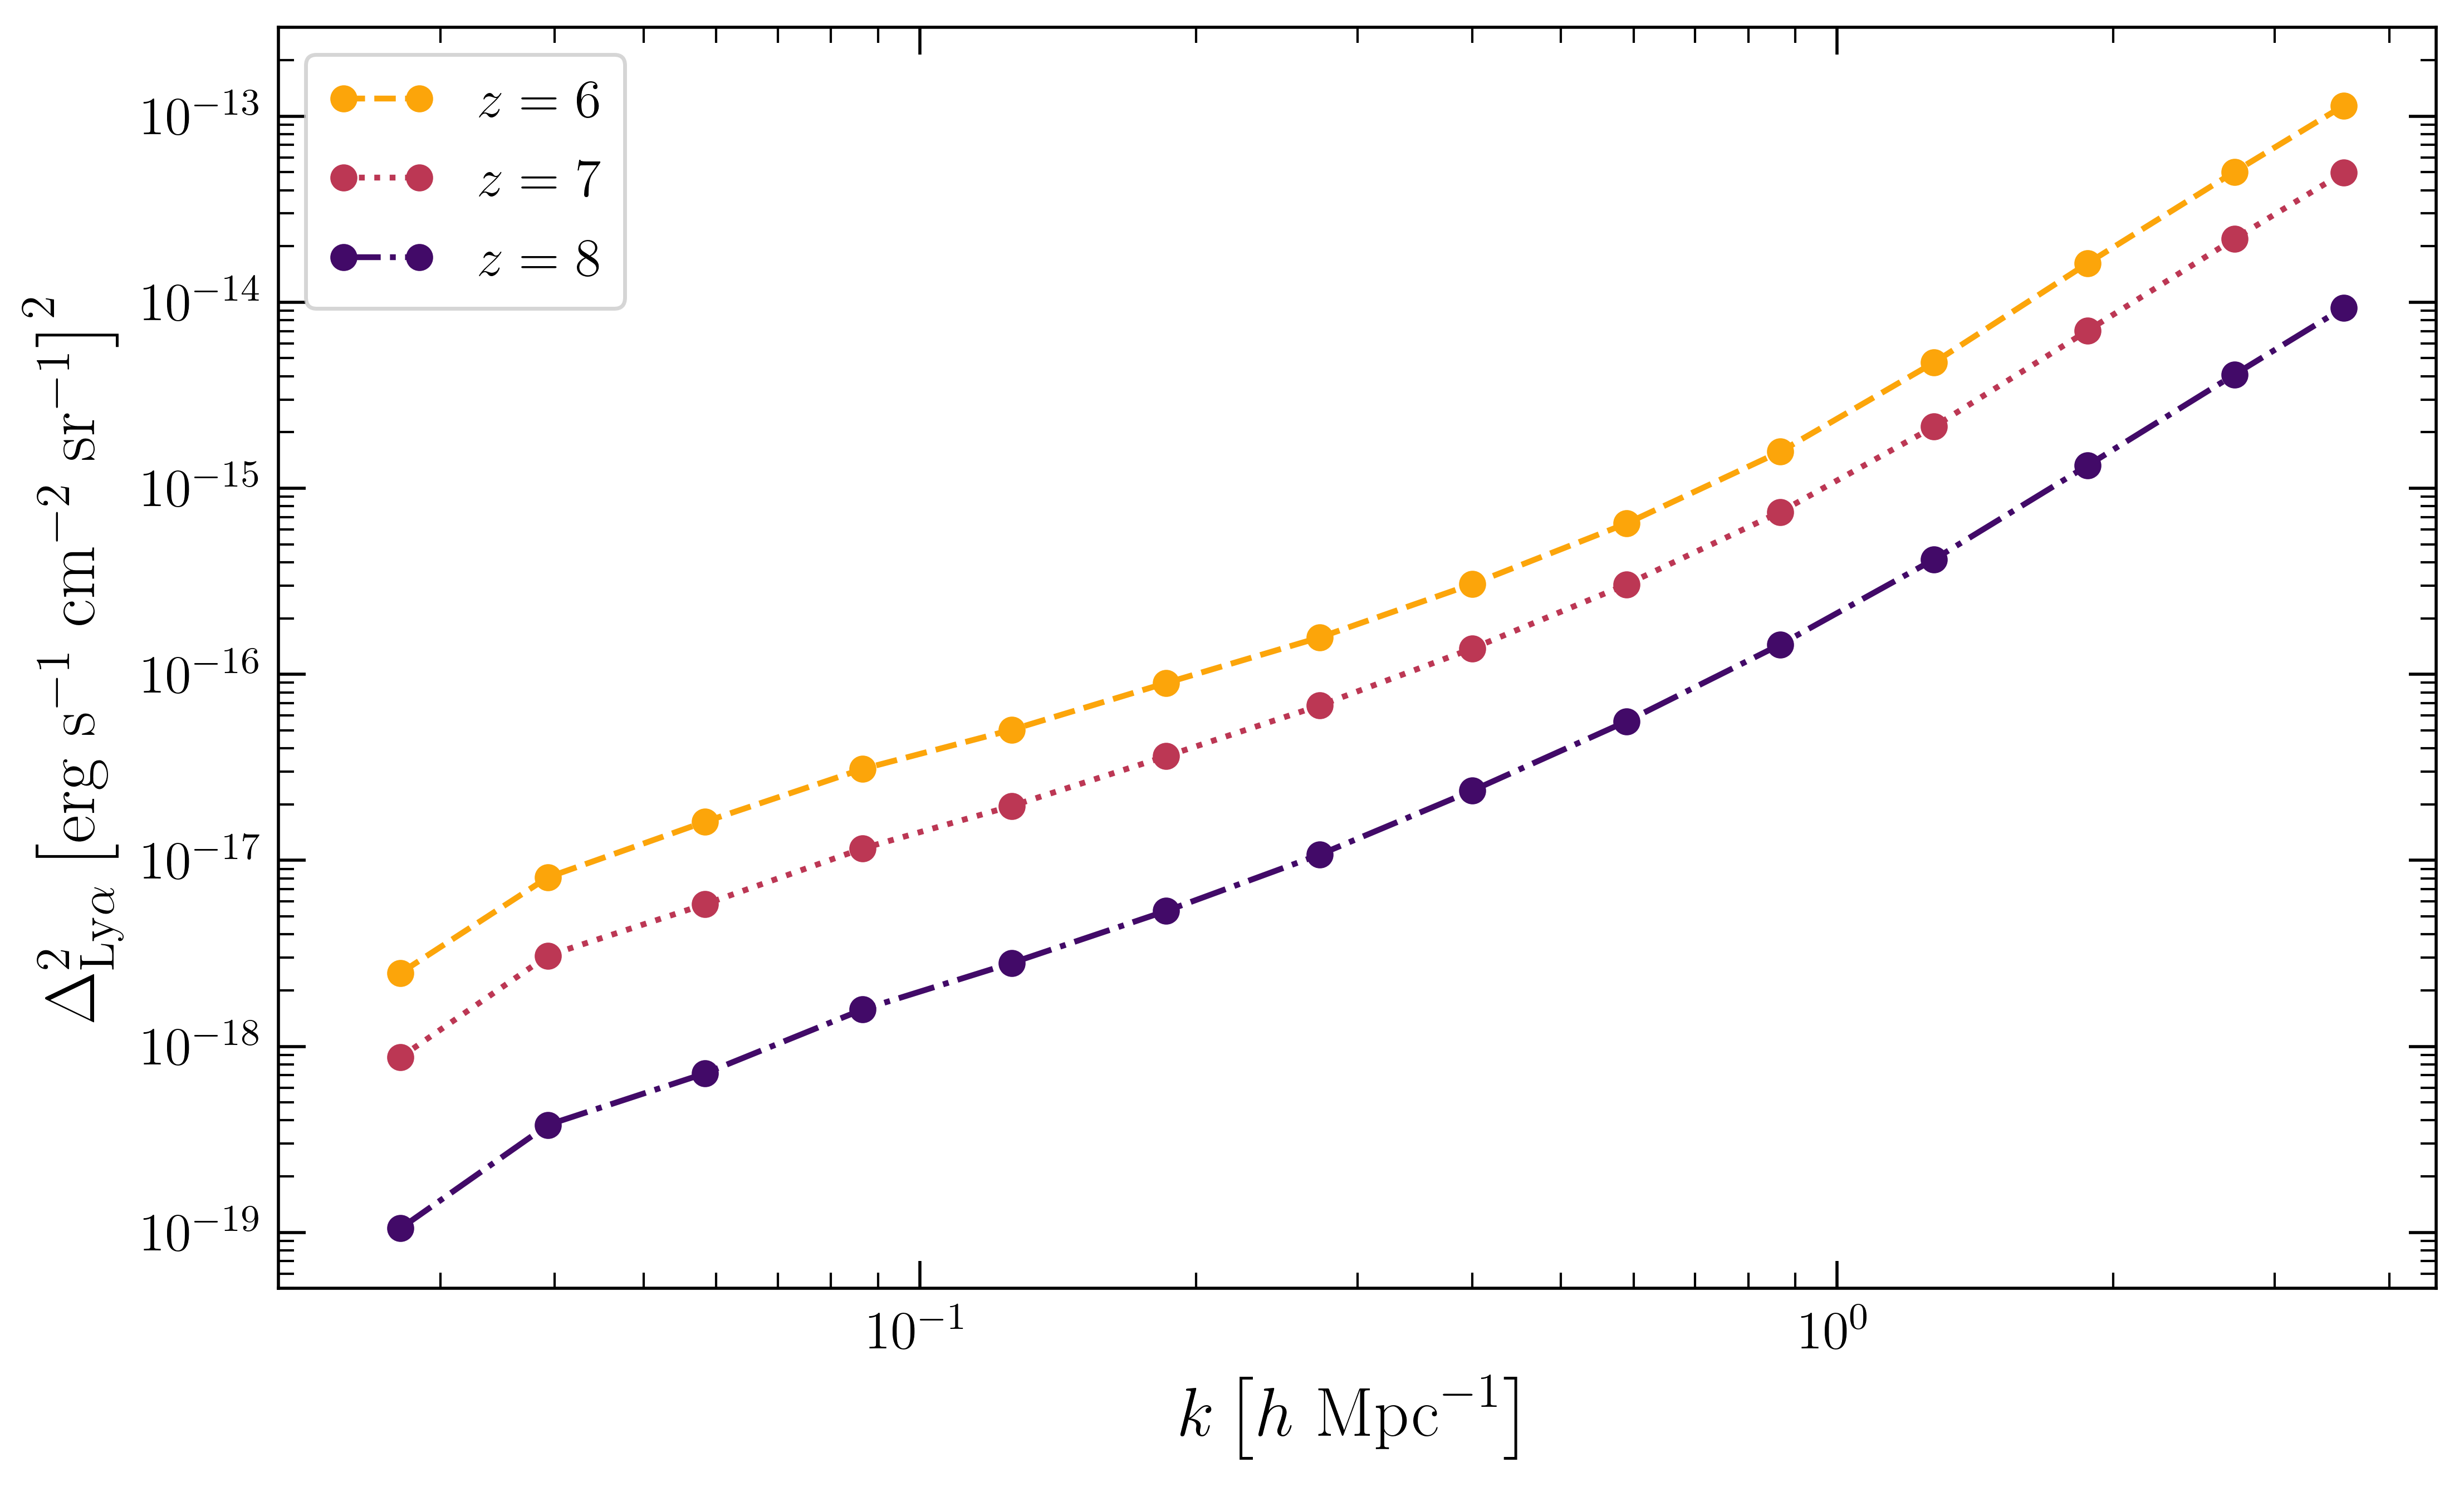
\includegraphics[width=0.9\textwidth]{lyman_alpha_pspec.png}
	\caption[Ly$\alpha$ Power Spectrum]{Cross-correlation coefficient}
	\label{fig:lya_ps}
\end{figure}

\begin{figure}[ht]
	\centering
	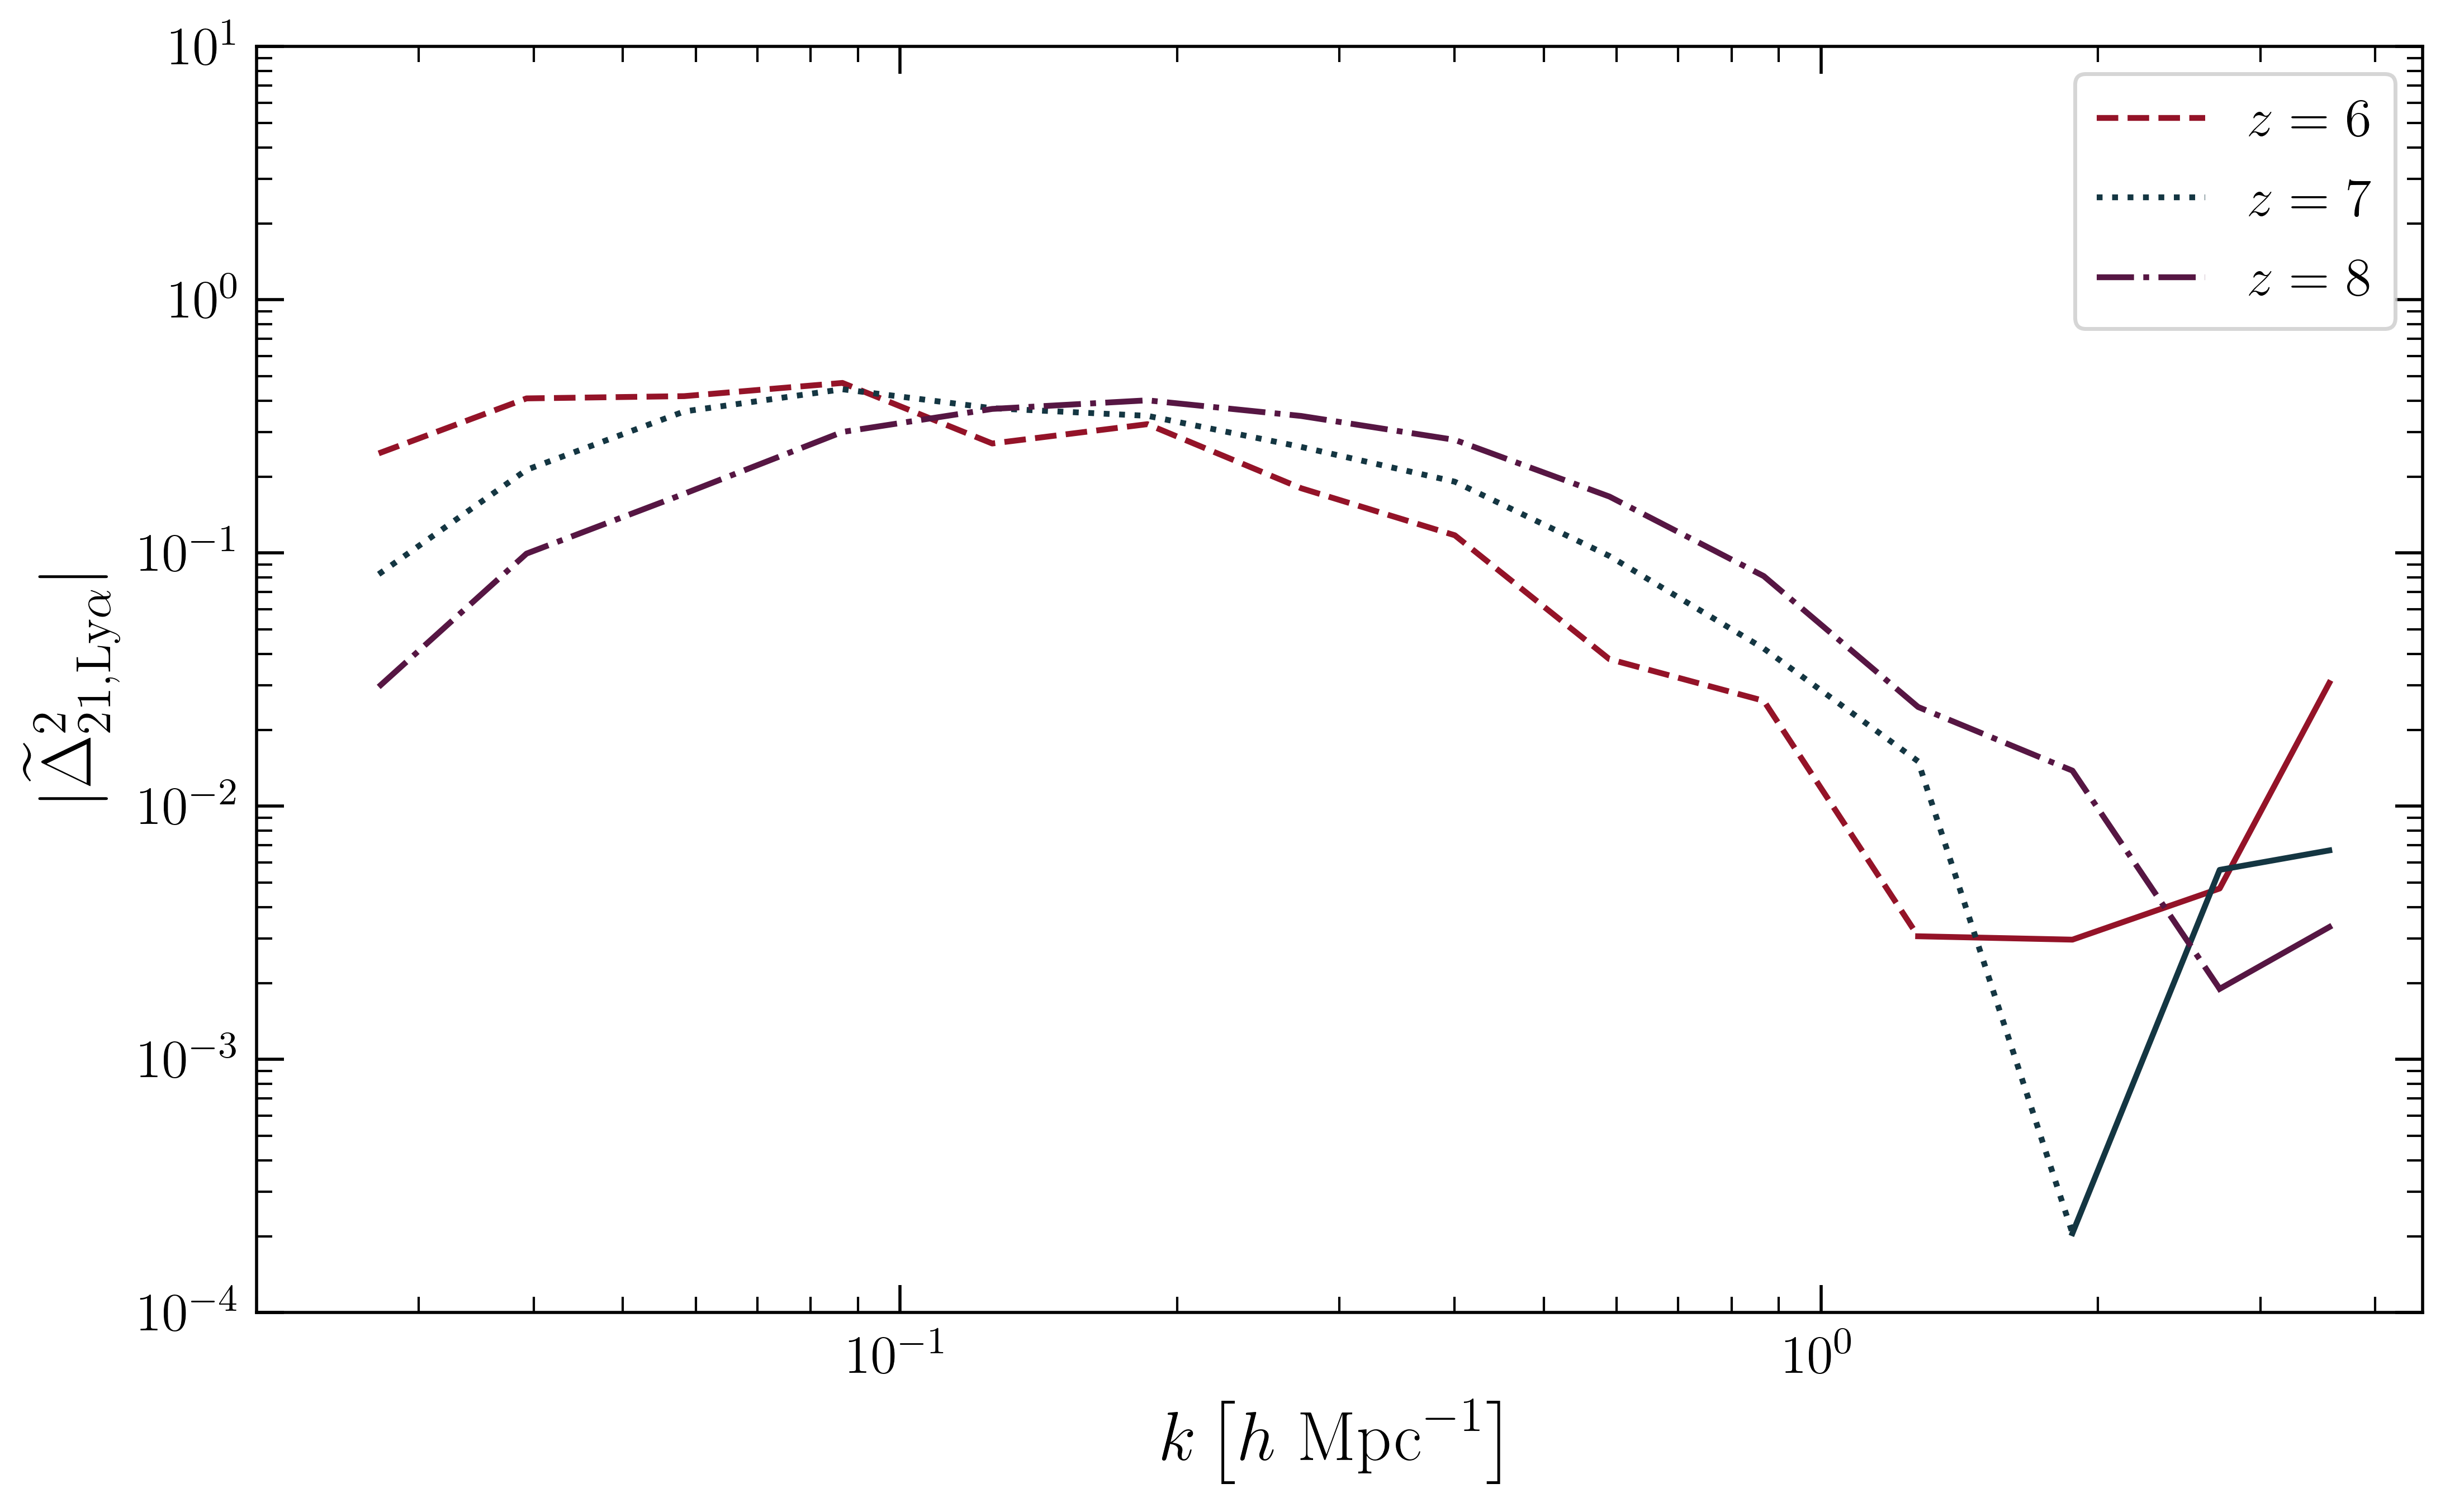
\includegraphics[width=0.9\textwidth]{cross_power_spec.png}
	\caption[Cross-Power Spectrum]{Cross-correlation coefficient}
	\label{fig:x_ps}
\end{figure}

\begin{figure}[ht]
	\centering
	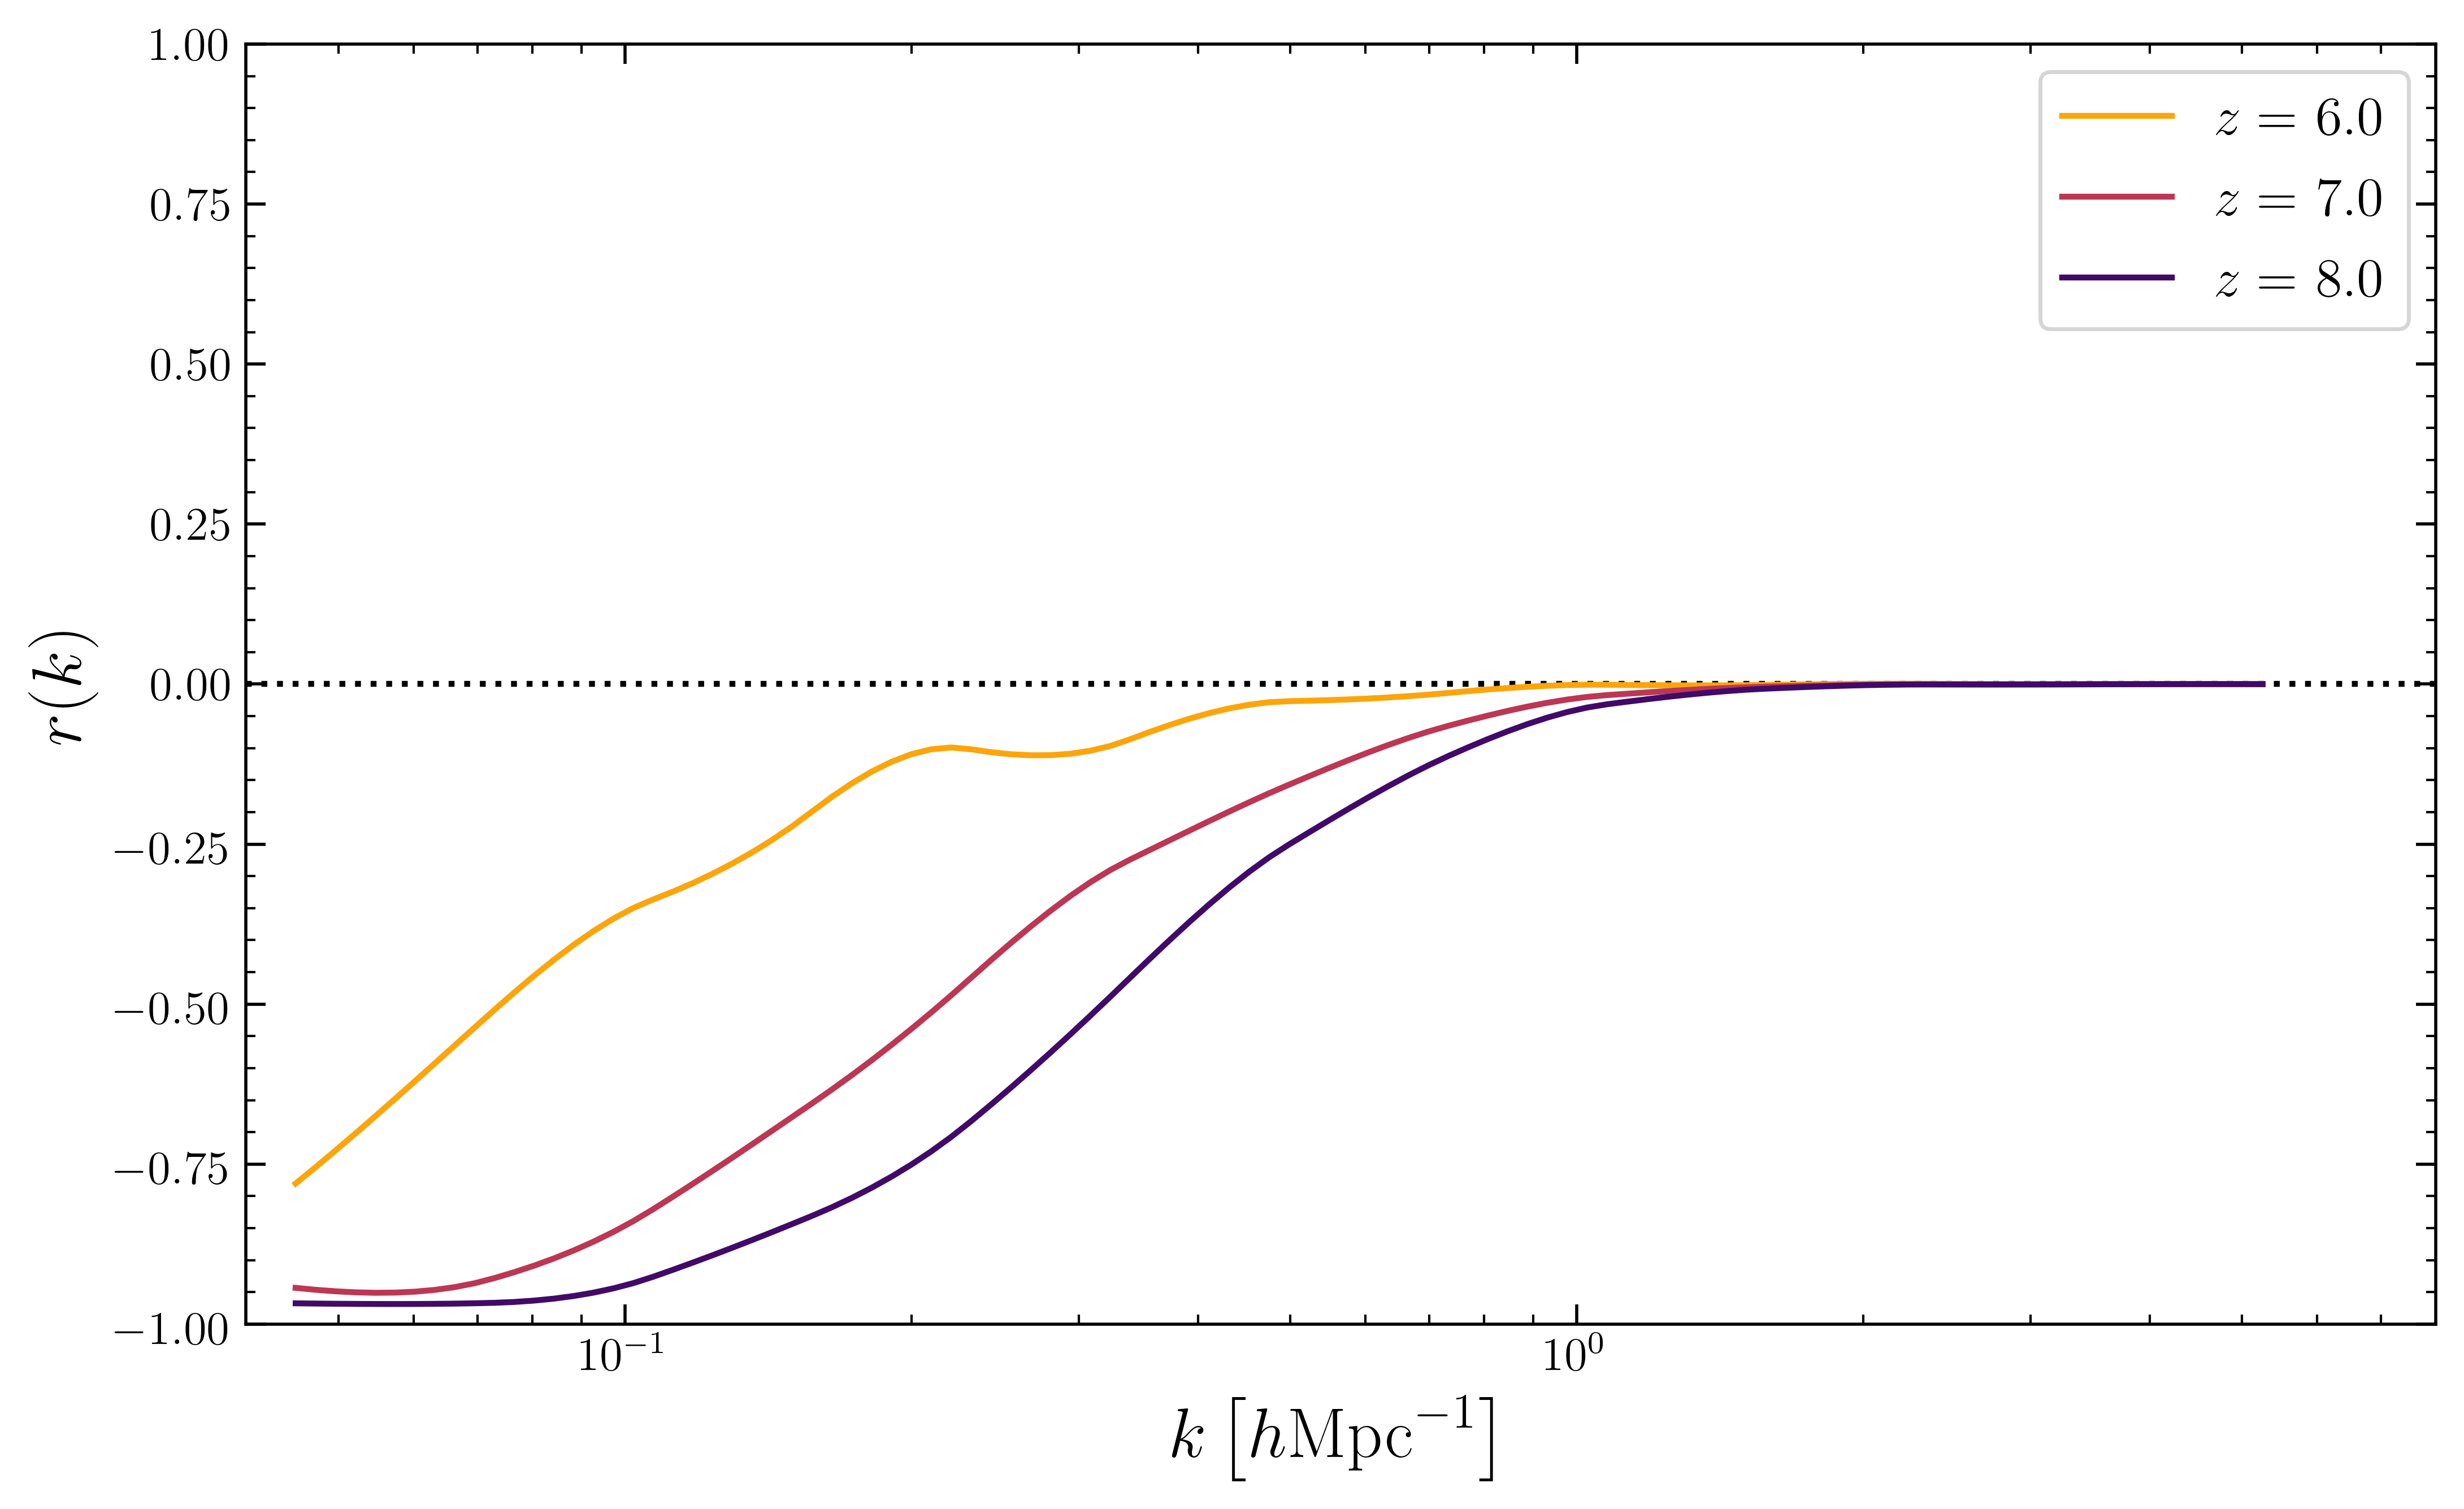
\includegraphics[width=0.9\textwidth]{ccc_plot.png}
	\caption[Cross-Correlation Coefficient]{Cross-correlation coefficient}
	\label{fig:ccc}
\end{figure}


	\tocless\subsection{\hypertarget{subsec:results}{3.2.\hspace{0.75em}Observational Uncertainties}}
	\addcontentsline{toc}{subsection}{3.2.\hspace{0.75em}Observational Uncertainties}

		21cm uncertainty

\begin{equation}
\sigma_{21}^2 = \left[ P_{21}\left(k_{\perp}, k_{\parallel} \right) + \frac{T^2_{\rm sys} V_{\rm sur}}{B \ t_{\rm int} \ n \left(k_{\perp}\right)} \right]
\end{equation}

\begin{equation}
V_{\rm sur} = D^2 \Delta D \left( \lambda_{21}^2 \left( z \right) / A_e\right)^2
\end{equation}


Ly$\alpha$ uncertainty

\begin{equation}
P_{N, \rm Ly\alpha} = \sigma_{\rm N}^2 V_{\rm vox} {\rm W}_{\rm Ly\alpha}\left(k, \mu \right)
\end{equation}

$V_{\rm vox} = A_{\rm pix} r_{\rm pix}$

\begin{equation}
\sigma_{\rm Ly\alpha} = \left[ P_{\rm Ly\alpha}\left(k, \mu \right) + P_{N, \rm Ly\alpha} \right]
\end{equation}

21cm-Ly$\alpha$ uncertainty


\begin{equation}
    2 \sigma^2_{21, \rm Ly\alpha} = P^2_{21, \rm Ly\alpha} + \sigma_{21} \sigma_{\rm Ly\alpha}
\end{equation}

\begin{equation}
\frac{1}{\sigma^2 \left( k \right)} = \sum_{\mu} \frac{N_{\rm m}}{\sigma^2 \left( k, \mu \right)}
\end{equation}


	\tocless\subsection{\hypertarget{subsec:results}{3.3.\hspace{0.75em}Foreground Contamination}}
	\addcontentsline{toc}{subsection}{3.3.\hspace{0.75em}Foreground Contamination}

		\begin{equation}
    k_{\parallel} \lesssim  \theta \frac{D_{M}\left( z \right) E \left( z \right)}{D_H \left(1 + z\right)} k_{\perp}
\end{equation}

\begin{equation}
    \theta = 1.22 \frac{\lambda}{D}
\end{equation}

Here is an explanation of the wedge

Cross correlation of cosmological 21cm observations with Ly$\alpha$ intensity
mapping surveys have the advantage that 21cm foregrounds do not correlation with
the foregrounds. Because the two do not correlate, no power from the foregrounds
is added to the cross-power spectrum. However, while the foregrounds don't contribute
to the total cross-power spectrum, they do contribute to the overall variance
of the measurement, and therefore the errors.

In the previous section, I calculated the cross-power spectrum for the case where
foreground are completely uncorrelated (don't contribute to the cross-power spectrum
amplitude) and where they did not contribute to the total variance. In this section,
I'll take a more realistic and honest approach to calculating the errors by dealing
with the 21cm foregrounds in two different ways. There are two primary methods
that I chose to deal with the foregrounds: by relying on the fact that the foregrounds
are spectrally smooth and thus confined to an area of the 2D power spectrum known
as the wedge and by assuming some imperfect removal method. Each method has advantages
and disadvantages.

In addition to avoiding 21cm foregrounds by cutting out k-modes that fall within
the wedge, efforts are being made to model 21cm point sources and foregrounds to
directly remove them from the data. This technique is known as foreground subtraction.
While this modeling foregrounds accurately has been shown to be quite difficult,
it gives the added benefit of recovering the foreground modes that fall within
the wedge, increasing the signal to noise of the measurement, assuming perfect (or
near perfect) foreground subtraction.

While outside the scope of this particular project, foreground subtraction could
be a viable method for recovering k-modes afflicated by bright 21cm foregrounds
and potentially allow for higher signal to noise measurements of the cross power
spectrum, given sufficient enough subtraction.

I plan to incorporate a treatment of the foreground subtraction in future works.
Previous works have handled the modeling of the power spectrum due to bright

\begin{equation}
    P_F \left(q, y\right) = \sum_{j} \epsilon_j^2 A_j \left( \frac{l}{2 \pi q} \right)^{n_j} \left( \frac{\nu_p}{\nu_i}\right)^{m_j}
\end{equation}

The total variance on the 21cm-Ly$\alpha$ cross power spectrum measurements would
then be written as:

\begin{equation}
    2 \sigma^2_{21, \rm Ly\alpha} = P^2_{21, \rm Ly\alpha} +
      \left(P_{21} + P_{F} + \sigma_{21} \right) \left( P_{\rm Ly\alpha} + \sigma_{\rm Ly\alpha}\right)
\end{equation}



		%----------------------------------%
		%							Conclusions	  			 %
		%----------------------------------%

\tocless\section{\hypertarget{sec:summary}{4.\hspace{0.75em}Conclusions}}
\addcontentsline{toc}{section}{4.\hspace{0.75em}Conclusions}

This is where my smart words go. I'll say very smart things here. \fastsim

\newpage
\tocless\section{\hypertarget{references}{References}}
\addcontentsline{toc}{section}{References}
\bibliographystyle{aasjournal}
\nocite{*}
\bibliography{refs}

\newpage
\tocless\section{\hypertarget{appendix}{Appendix}}
\addcontentsline{toc}{section}{Appendix}

This is where appendix-y things go


\end{document}
